%%%%%%%%%%%%%%%%%%%%%%%%%%%%%%%%%%%%%%%%%
% 
% PSI Chair Thesis Template
% Version 2019-12
% 
% based on MastersDoctoralThesis.cls
% Version 2.5 (27/8/17)
%
% which was obtained from:
% http://www.LaTeXTemplates.com
%
% Version 2.x major modifications by:
% Vel (vel@latextemplates.com)
%
% This template is based on a template by:
% Steve Gunn (http://users.ecs.soton.ac.uk/srg/softwaretools/document/templates/)
% Sunil Patel (http://www.sunilpatel.co.uk/thesis-template/)
%
% Template license:
% CC BY-NC-SA 3.0 (http://creativecommons.org/licenses/by-nc-sa/3.0/)
%
%%%%%%%%%%%%%%%%%%%%%%%%%%%%%%%%%%%%%%%%%

%----------------------------------------------------------------------------------------
%	PACKAGES AND OTHER DOCUMENT CONFIGURATIONS
%----------------------------------------------------------------------------------------

\PassOptionsToPackage{english,ngerman}{babel}
\documentclass[
11pt, % The default document font size is 11 (recommended), options: 10pt, 11pt, 12pt
%oneside, % Two-side layout isrecommended; uncomment to switch to one-sided
english, % replace with ngerman for German; not fully supported so far -- requires changes elsewhere
singlespacing, % Single line spacing (recommended), alternatives: onehalfspacing or doublespacing
%draft, % Uncomment to enable draft mode (no pictures, no links, overfull hboxes indicated)
%nolistspacing, % If the document is onehalfspacing or doublespacing, uncomment this to set spacing in lists to single
%liststotoc, % Uncomment to add list of figures/tables/etc to table of contents (not recommended)
%toctotoc, % Uncomment to add the main table of contents to the table of contents (not recommended)
parskip, % add space between paragraphs (recommended)
nohyperref, % do not load the hyperref package (is loaded in setup.tex)
headsepline, % print a horizontal line under the page header
consistentlayout, % layout of declaration, abstract and acknowledgements pages matches the default layout
%final, % Uncomment to hide all todo notes
]{PsiThesis} % The class file specifying the document structure


%----------------------------------------------------------------------------------------
%		UNIVERSITY OF BAMBERG COLORS
%----------------------------------------------------------------------------------------

% http://www.brandwares.com/RGBTintCalculator.php
% Base Color value obtained from UB Corporate Identity Manual 
\definecolor{ubblue}{HTML}{00457D}
\definecolor{ubblue80}{HTML}{336A97}
\definecolor{ubblue60}{HTML}{668FB1}
\definecolor{ubblue40}{HTML}{99B5CB}
\definecolor{ubblue20}{HTML}{CCDAE5}

\definecolor{ubyellow}{HTML}{FFD300}
\definecolor{ubyellow25}{HTML}{FFF4BF}

\definecolor{ubred}{HTML}{e6444F}

\definecolor{ubgreen}{HTML}{97BF0D}

\definecolor{gray75}{gray}{0.75}
\definecolor{gray50}{gray}{0.50}

%----------------------------------------------------------------------------------------
%		FONT SETUP
%----------------------------------------------------------------------------------------

\usepackage[T1]{fontenc} % Output font encoding for international characters
\usepackage[utf8]{luainputenc} % makes unicode characters like –, €, and ß work properly

\usepackage{fontspec} % allows us to use OTF/TTF fonts

% If you cannot use the cochineal font, uncomment the following lines to select
% the Crimson font. Note, however, that you'll have to take care of the math font
% on your own.
% 
%\setmainfont[
%	Path           = fonts/,
%    BoldFont       = {Crimson-Semibold.otf},
%    ItalicFont     = {Crimson-Italic.otf},
%    BoldItalicFont = {Crimson-BoldItalic.otf}
%]{Crimson-Roman.otf}

% Recommended: use Cochineal with old-style figures (math fonts: see further down)
\usepackage[p,osf]{cochineal}
 
% Exception: tables should use "lining figures" (all digits having same width)
\AtBeginEnvironment{tabular}{%
  \tlfstyle
}
\AtBeginEnvironment{tabularx}{%
  \tlfstyle
}

% monospace font, will be used in verbatim and listing environments
\setmonofont[
	Path           = fonts/,
    BoldFont       = {UbuntuMono-B.ttf},
    ItalicFont       = {UbuntuMono-RI.ttf},
    BoldItalicFont       = {UbuntuMono-BI.ttf},
    Scale = 0.92 % manually determined value; MatchLowercase does not work with Cochineal because it is not included loaded via fontspec
]{UbuntuMono-R.ttf}

% sans-serif font, will be used in the margins
\setsansfont[
	Path          	= fonts/,
	BoldFont		= Roboto-Bold.otf,
	ItalicFont		= Roboto-Italic.otf,
	BoldItalicFont	= Roboto-BoldItalic.otf,
	Scale = 0.83 % manually determined value; MatchLowercase does not work with Cochineal because it is not included loaded via fontspec
]{Roboto-Regular.otf}

\renewcommand{\familydefault}{\rmdefault}
\defaultfontfeatures{Ligatures=TeX}

% math fonts that go well with cochineal 
\usepackage[cochineal,vvarbb]{newtxmath}
\usepackage[cal=boondoxo]{mathalfa}


%----------------------------------------------------------------------------------------
%		HEADINGS SETUP (CHAPTERS, SECTIONS, …)
%----------------------------------------------------------------------------------------

% ====== replace Q with \Qswash in Chapters and Sections =========
\newcommand{\swashedletter}{\Qswash}
\catcode`Q=\active
\defQ{\swashedletter}
\catcode`Q=11
\usepackage{xstring}
\noexpandarg\exploregroups
\newcommand\ReplaceStrQ[1]{\StrSubstitute{#1}{Q}{\swashedletter}}
% ================================================================

\usepackage[explicit]{titlesec}
\newcommand{\hsp}{\hspace{20pt}}

\setcounter{secnumdepth}{3}

% chapters have a vertical line between number and title
\titleformat{\chapter}[hang]{\Huge\bfseries}{\color{ubblue60}\thechapter}{20pt}{\begin{tabular}[t]{@{\color{ubblue60}\vrule width 2pt\hsp}p{0.85\textwidth}}\raggedright\ReplaceStrQ{#1}\end{tabular}}

% sections
\titleformat{\section}[hang]{\bfseries\large}{{\color{ubblue80}\thechapter.\arabic{section}}}{1ex}{{\color{ubblue80}\ReplaceStrQ{#1}}}{}

% subsections
\titleformat{\subsection}[hang]{\bfseries\large}{{\color{ubblue80}\thechapter.\arabic{section}.\arabic{subsection}}}{1ex}{{\color{ubblue80}\ReplaceStrQ{#1}}}{}

% subsubsections
\titleformat{\subsubsection}[hang]{\bfseries}{{\color{ubblue80}\thechapter.\arabic{section}.\arabic{subsection}.\arabic{subsubsection}}}{1ex}{{\color{ubblue80}\ReplaceStrQ{#1}}}{}

% vertical spacing for headings ==============
\titlespacing*{\section}
{0pt}{7ex}{3ex}

\titlespacing*{\subsection}
{0pt}{4ex}{2ex}

\titlespacing*{\subsubsection}
{0pt}{4ex}{2ex}
% end of vertical spacing ====================

%----------------------------------------------------------------------------------------
%		TABLE OF CONTENTS SETUP
%----------------------------------------------------------------------------------------

% solution inspired from https://tex.stackexchange.com/questions/178510/how-can-i-reproduce-this-beautiful-table-of-contents
\usepackage{etoc}
\etocsetlevel{section}{2}
\etocsetlevel{subsection}{3}

\etocsettocdepth{section} % set to subsection for adding subsections to toc (not recommended)

\newlength{\tocleft}
\setlength{\tocleft}{2.5cm} % must be set to fit the innermargin defined in geometry (change only if you have changed the margins)

\newlength{\tocsep}
\setlength{\tocsep}{2em}

\usepackage{textcase}

\etocsetstyle{chapter}
   {}
   {}
   {\etocifnumbered
     {\makebox[0pt][r]
       % we use \etocthenumber instead of \etocnumber to avoid the href, which is part of \etocthenumber, messing with MakeTextLowercase
       {\textsc{\MakeTextLowercase\chaptername\ \MakeTextLowercase\etocthenumber}\hspace{\tocsep}}%
       \textbf{\etocname\kern1em\relax\etocpage}%
    }%
    {\textbf{\etocname\kern1em\relax\etocpage}}%
    \par\vspace{3ex}%
   }%
   {}

\etocsetstyle{section}
   {\vspace{-2ex}} % Muss von den 3ex aus Chapter abgezogen werden
   {}
   % see the comment regarding etocthenumber in the chapter style definition
   {\makebox[0pt][r]{\textsc{\MakeTextLowercase\etocthenumber}\hspace{\tocsep}}%
    \etocname\kern1em\etocpage\par%
   }%
   {\addvspace{3ex}} % 3ex falls danach Chapter kommt 

\etocsetstyle{subsection} 
   {\vspace{0ex}} 
   {} 
   {\makebox[3em][l]{\etocnumber}\etocname\kern1em\etocpage\par} 
   {\addvspace{2ex}} % 2ex falls danach Section kommt 

\etocsettocstyle{\chapter*{\contentsname}
                \thispagestyle{plain}%
                \leftskip\tocleft\parindent0pt}{}


%----------------------------------------------------------------------------------------
%		OTHER PACKAGES
%----------------------------------------------------------------------------------------

\usepackage{tabularx} % for more flexible tables

\usepackage{marginnote} % Enable Notes on the Page Margin
\usepackage{ragged2e} % provides better hyphenation, use with camel case: \RaggedRight 
\renewcommand*{\raggedleftmarginnote}{\RaggedLeft}
\renewcommand*{\raggedrightmarginnote}{\RaggedRight}
\renewcommand*{\marginfont}{\setlength{\parskip}{0.5ex}\scriptsize\sffamily} % format margin text



% for sidenotes: change marginpar font
\usepackage{xparse}
\let\oldmarginpar\marginpar
\RenewDocumentCommand{\marginpar}{om}{%
  \IfNoValueTF{#1}
    {\oldmarginpar{\mymparsetup #2}}
    {\oldmarginpar[\mymparsetup #1]{\mymparsetup #2}}}
\newcommand{\mymparsetup}{\scriptsize\sffamily}


% this provides correct alignment for margin text that is inserted
% right at the beginning of a paragrah; however, it messes up the
% alignment in all other cases.
%% therefore, removed for now:
%%\renewcommand{\marginnotevadjust}{0.71\baselineskip}
% The following is the necessary correction for in-paragraph use
\renewcommand{\marginnotevadjust}{0.21\baselineskip} 
\renewcommand{\marginnotevadjust}{0.55\baselineskip}

\usepackage{microtype} % enable better typographic setup

\usepackage{multicol} % enable usage of multiple columns

% biblatex setup
% inspired by https://anneurai.net/2017/10/18/thesis-formatting-in-latex/
\usepackage[
  backend=biber,
  style=alphabetic,
  doi=false,isbn=false, % these fields are commonly omitted
  terseinits=true, % no points between initials
  giveninits=true, % always print only initials for given names
  sortcites=true,
  language=english,
  backref=true, % show on what pages a ref has been cited
]{biblatex} % Use biber backend with alphabetic reference style
\AtEveryBibitem{%
  \clearlist{language} % don't show "en."
  \clearlist{extra} % clears extra fields such as ISBN nrs
}

% shorten the strings used in back references
\DefineBibliographyStrings{english}{%
  backrefpage = {page},
  backrefpages = {pages},
}

%-- no "quotes" around titles of chapters/article titles
\DeclareFieldFormat[article, inbook, incollection, inproceedings, misc, thesis, unpublished]{title}{#1}
%-- no punctuation after volume
\DeclareFieldFormat[article]{volume}{{#1}}
%-- puts number/issue between brackets
\DeclareFieldFormat[article, inbook, incollection, inproceedings, misc, thesis, unpublished]{number}{\mkbibparens{#1}}
%-- and then for articles directly the pages w/o any "pages" or "pp."
\DeclareFieldFormat[article]{pages}{#1}
%-- format 16(4):224--225 for articles
\renewbibmacro*{volume+number+eid}{\printfield{volume}\printfield{number}\printunit{\addcolon}
}
\DeclareFieldFormat{url}{\url{#1}}


\usepackage[autostyle=true]{csquotes} % Required to generate language-dependent quotes in the bibliography

\usepackage[
  obeyFinal,
  textsize=scriptsize,
  backgroundcolor=ubyellow25,linecolor=ubyellow,bordercolor=ubyellow,
]{todonotes}

% change font of todo notes to sans-serif
\makeatletter
\renewcommand{\todo}[2][]{\@bsphack\@todo[#1]{\sffamily #2}\@esphack\ignorespaces}
\makeatother

\usepackage{booktabs} % use formal table layout

\urlstyle{same} % avoids printing URLs in typewriter font

% enable very extensive URL breaking
% https://tex.stackexchange.com/questions/3033/forcing-linebreaks-in-url
\PassOptionsToPackage{hyphens}{url}
\expandafter\def\expandafter\UrlBreaks\expandafter{\UrlBreaks% save the current one
  \do\a\do\b\do\c\do\d\do\e\do\f\do\g\do\h\do\i\do\j%
  \do\k\do\l\do\m\do\n\do\o\do\p\do\q\do\r\do\s\do\t%
  \do\u\do\v\do\w\do\x\do\y\do\z\do\A\do\B\do\C\do\D%
  \do\E\do\F\do\G\do\H\do\I\do\J\do\K\do\L\do\M\do\N%
  \do\O\do\P\do\Q\do\R\do\S\do\T\do\U\do\V\do\W\do\X%
  \do\Y\do\Z\do\*\do\-\do\~\do\'\do\"\do\-}%

% TODO consider using package xurl, which is supposed to handle urL breaking 

% https://tex.stackexchange.com/a/450695
% allow URLs to be spaced out at / => much better URL breaking in margins
\makeatletter
\g@addto@macro\UrlSpecials
{%
    \do\/{\mbox{\UrlFont/}\hskip 0pt plus 2pt}%
}
\Urlmuskip=0mu plus 1mu\relax
\makeatother


% hyperlink layout
\usepackage{hyperref}
 \hypersetup{colorlinks,breaklinks,unicode,
             citecolor=ubblue60,
             linkcolor=ubblue60,
             filecolor=ubblue60,
             urlcolor=ubblue60}


% should make links appear in black when PDF is printed
% (do not use, breaks title page layout)
%\usepackage[ocgcolorlinks]{ocgx2}

% cleverref allows you to use |Cref{sec:foo} to get the text "Section 1.2".
% This also works with figures and tables.
\usepackage{cleveref}

\raggedbottom % do NOT force all pages to have the same height (which would be done by increasing the space between paragraphs, which can create noisy layouts)

%----------------------------------------------------------------------------------------
%	SETUP BIBLIOGRAPHY
%----------------------------------------------------------------------------------------
\setlength{\bibitemsep}{.3\baselineskip plus .05\baselineskip minus .05\baselineskip}
\newlength{\bibparskip}\setlength{\bibparskip}{0pt}
\let\oldthebibliography\thebibliography
\renewcommand\thebibliography[1]{%
  \oldthebibliography{#1}%
  \setlength{\parskip}{\bibitemsep}%
  \setlength{\itemsep}{\bibparskip}%
}

% allow much more liberal line breaks in URLs
\setcounter{biburllcpenalty}{7000}
\setcounter{biburlucpenalty}{8000}

% adjust space between key and entry, default is 2\labelsep
\setlength{\biblabelsep}{1\labelsep} 

% configures indentation of bibentries
\defbibenvironment{bibliography}
  {\list
     {\hspace{0.5\labelalphawidth}\bfseries\printtext[labelalphawidth]{%
        \printfield{prefixnumber}%
        \printfield{labelalpha}%
        \printfield{extraalpha}}}
     {\setlength{\labelsep}{\biblabelsep}%
      \setlength{\leftmargin}{0.5\labelalphawidth}%
      \setlength{\itemsep}{1.5\bibitemsep}%
      \setlength{\parsep}{\bibparsep}}%
      \renewcommand*{\makelabel}[1]{##1\hss}}
  {\endlist}
  {\item}


%----------------------------------------------------------------------------------------
%	MARGIN SETTINGS
%----------------------------------------------------------------------------------------

%\geometry{
%	paper=a4paper, % Change to letterpaper for US letter (not recommended)
%	inner=2cm, % Inner margin
%	outer=6.2cm, % Outer margin, extra wide for margin notes
%	marginparwidth=4cm,
%	marginparsep=4mm,
%	bindingoffset=.5cm, % Binding offset
%	top=2.0cm, % Top margin
%	bottom=2.5cm, % Bottom margin
%	% showframe, % Uncomment to show how the type block is set on the page
%}

% testing, from kaobook
\geometry{
		paper=a4paper,
		top=27.4mm,
		bottom=27.4mm,
		inner=24.8mm,
		%outer=24.8mm,
		%right=2.183cm,
		textwidth=107mm,
		marginparsep=8.2mm,
		marginparwidth=49.4mm,
		%textheight=49\baselineskip,
		includemp,
		% showframe
}

% Wide figures span text and margin.
% Use the pre-calculated length \widefigurewidth in \includegraphics.
\def\widefigurewidth{\dimexpr(\marginparwidth + \textwidth + \marginparsep)}

%----------------------------------------------------------------------------------------
%	SETUP HEADER AND FOOTER
%----------------------------------------------------------------------------------------


\newlength{\overflowingheadlen}
\setlength{\overflowingheadlen}{\textwidth}
\addtolength{\overflowingheadlen}{\marginparsep}
\addtolength{\overflowingheadlen}{\marginparwidth}

% old header/footer, maybe not necessary any more?
\automark[chapter]{chapter}
\ihead{\textup{\headmark}} % Inner header; do not use italics: therefore textup
\ihead{\textup{\textsc{\MakeLowercase\headmark}}}% Inner header - use this line for Small Caps in header
\ohead[]{\pagemark} % Outer header
\cfoot[\pagemark]{} % On chapter opening pages, the page number goes centered into the footer
\automark*[section]{}%

% new header/footer, from kaobook; we could probably remove the original definitions from the cls
\renewpagestyle{thesis}{
  {\hspace{-\marginparwidth}\hspace{-\marginparsep}\makebox[\overflowingheadlen][l]{\thepage\quad\rule[-\dp\strutbox]{1pt}{\baselineskip}\quad{}\textup{\textsc{\MakeLowercase \leftmark}}}}%
  {\makebox[\overflowingheadlen][r]{\textup{\textsc{\MakeLowercase \rightmark}}\quad\rule[-\dp\strutbox]{1pt}{\baselineskip}\quad\thepage}}%
  {}
}{
  {}%
  {}%
  {}
}
\renewpagestyle{plain.thesis}{
  {}%
  {}%
  {}
}{
  {\thepage}%
  {\makebox[\overflowingheadlen][r]{\rule[-\dp\strutbox]{1pt}{\baselineskip}\quad\thepage}}%
  {}
}

%----------------------------------------------------------------------------------------
%	LISTINGS SETTINGS
%----------------------------------------------------------------------------------------

\usepackage{textcomp}
\usepackage{listings}
\definecolor{darkgray}{rgb}{.4,.4,.4}

\lstdefinelanguage{JavaScript}{
  keywords={typeof, new, true, false, catch, function, return, null, catch, switch, var, if, in, while, do, else, case, break},
  ndkeywords={class, export, boolean, throw, implements, import, this},
  sensitive=false,
  comment=[l]{//},
  morecomment=[s]{/*}{*/},
  morestring=[b]',
  morestring=[b]"
}

\lstset{
    aboveskip={1\baselineskip},
    abovecaptionskip=-1\baselineskip,
    belowcaptionskip=2ex,
    basicstyle=\footnotesize\ttfamily\linespread{4},
    breaklines=true,
    columns=flexible,
    commentstyle=\color{gray50}\ttfamily\itshape,
    escapechar=@,
    extendedchars=true,
    frame=l,
    framerule=.7pt,
    identifierstyle=\color{black},
    inputencoding=latin1,
    keywordstyle=\color{ubblue80}\bfseries,
    ndkeywordstyle=\color{ubblue80}\bfseries,
    numbers=left,
    numbersep=1em,
    numberstyle=\scriptsize\tlfstyle,
    prebreak = \raisebox{0ex}[0ex][0ex]{\ensuremath{\hookleftarrow}},
    stringstyle=\color{ubblue60}\ttfamily,
    upquote=true,
    showstringspaces=false,
}

\lstset{literate=%
   *{0}{{{\color{darkgray}0}}}1
    {1}{{{\color{darkgray}1}}}1
    {2}{{{\color{darkgray}2}}}1
    {3}{{{\color{darkgray}3}}}1
    {4}{{{\color{darkgray}4}}}1
    {5}{{{\color{darkgray}5}}}1
    {6}{{{\color{darkgray}6}}}1
    {7}{{{\color{darkgray}7}}}1
    {8}{{{\color{darkgray}8}}}1
    {9}{{{\color{darkgray}9}}}1
}

\lstnewenvironment{latex}
    {\lstset{language=[LaTeX]TeX}}
    {}

%----------------------------------------------------------------------------------------
%	MARGINAL CAPTIONS
%----------------------------------------------------------------------------------------

\usepackage{sidenotes}
\usepackage{scrextend} % for ifthispageodd

% objective: instead of having the sidenode numbner in superscript, want something like 1:
\makeatletter
\ExplSyntaxOn
\RenewDocumentCommand \sidenotetext { o o +m }
{
  \IfNoValueOrEmptyTF{#1}
    {
      \@sidenotes@placemarginal{#2}{\thesidenote{}:~#3}
  \refstepcounter{sidenote}
}
    {\@sidenotes@placemarginal{#2}{#1{}:~#3}}
}
\ExplSyntaxOff
\makeatother

% objective: automatically justify sidecaptions to match the other marginnotes
% captions of marginfigures etc. shall always be raggedright
% solution from: https://tex.stackexchange.com/questions/358010/subfigures-break-figure-numbering-with-sidecaptions-from-sidenotes-package/358012#358012

\makeatletter
\DeclareCaptionJustification{outerragged}{\ifthispageodd{\RaggedRight}{\RaggedLeft}}

\DeclareCaptionStyle{sidecaption}{format=plain,font={scriptsize,sf},labelfont=bf,margin=0pt,singlelinecheck=true,justification=outerragged} 
\DeclareCaptionStyle{marginfigure}{format=plain,font={scriptsize,sf},labelfont=bf,margin=0pt,singlelinecheck=true}
\DeclareCaptionStyle{margintable}{format=plain,font={scriptsize,sf},labelfont=bf,margin=0pt,singlelinecheck=true}
\DeclareCaptionStyle{widefigure}[justification=centering]{format=plain,font=small,labelfont=bf,justification=RaggedRight,singlelinecheck=true}
\DeclareCaptionStyle{widetable}[justification=centering]{format=plain,font=small,labelfont=bf,justification=RaggedRight,singlelinecheck=true}
\makeatother


%----------------------------------------------------------------------------------------
%	SYMBOLS
%----------------------------------------------------------------------------------------

\usepackage{pifont}
\let\oldding\ding% Store old \ding in \oldding
\renewcommand{\ding}[2][1]{\scalebox{#1}{\oldding{#2}}}% Scale \oldding via optional argument
% usage \ding{number} or |ding[factor]{number}

\usepackage{amssymb}

%----------------------------------------------------------------------------------------
%	ITEMIZE AND ENUMERATE ENVIRONMENTS
%----------------------------------------------------------------------------------------

\renewcommand{\labelitemi}{\color{ubblue80}{\scalebox{0.8}{\raisebox{0.2ex}{$\blacktriangleright$}}}}
\renewcommand{\labelitemii}{\textbullet}
\usepackage{enumitem}
\setlist[itemize]{parsep=0.8\parskip,left=0pt,topsep=0pt,partopsep=0pt}
\setlist[enumerate]{parsep=0.8\parskip,left=0pt,topsep=0pt,partopsep=0pt}
\setlist[description]{parsep=0.8\parskip,left=0pt,topsep=0pt,partopsep=0pt}


%----------------------------------------------------------------------------------------
%	SET PDF METADATA
%----------------------------------------------------------------------------------------

\AtBeginDocument{
\hypersetup{pdftitle=\ttitle} % Set the PDF's title to your title
\hypersetup{pdfauthor=\authorname} % Set the PDF's author to your name
%\hypersetup{pdfkeywords=\keywordnames} % Set the PDF's keywords to your keywords
}


\addbibresource{literature.bib} % The filename of the bibliography

%----------------------------------------------------------------------------------------
%	THESIS INFORMATION
%----------------------------------------------------------------------------------------
\newcommand{\thesistype}{Bachelors} % type of your thesis (Bachelors, Masters, Doctoral ...)
\newcommand{\abschluss}{Bachelor} % used in Declaration of Authorship (singular, German)

% This construct is used to replace the letter Q with \Qswash (defined in setup.tex) in title
\catcode`Q=\active
\defQ{\swashedletter}

%%% CHANGE THIS:
% Your thesis title, this is used in the title and abstract, print it elsewhere with \ttitle
\thesistitle{Just a Quick Example: This is a Thesis Title of Typical Length}

\catcode`Q=11 % make Q inactive again
%

%%% CHANGE THIS:
% Your name, this is used in the title page, print it elsewhere with \authorname
\author{Max Mustermann} 

% Your supervisor's name, this is used in the title page, print it elsewhere with \supname
\supervisor{Prof. Dr. Dominik Herrmann} 

% Your university's name and URL, this is used in the title page, print it elsewhere with \univname
\university{\href{https://www.uni-bamberg.de/en/}{University of Bamberg}}

% Your research group's name and URL, this is used in the title page, print it elsewhere with \groupname
\group{\href{https://www.uni-bamberg.de/en/psi/}{Privacy and Security in Information Systems Group}}

% Your department's name and URL, this is used in the title page, print it elsewhere with \deptname
\department{department not used}

% Your faculty's name and URL, this is used in the title page, print it elsewhere with \facname
\faculty{\href{https://www.uni-bamberg.de/en/wiai/}{Faculty of Information Systems and Applied Computer Sciences}}


% Your degree name, this is used in the title page, print it elsewhere with \degreename
\degree{degree not used}

% Your address, this is not currently used anywhere in the template, print it elsewhere with \addressname
\addresses{address not used}

% Your subject area, this is not currently used anywhere in the template, print it elsewhere with \subjectname
\subject{subject not used}

% Keywords for your thesis, this is not currently used anywhere in the template, print it elsewhere with \keywordnames
\keywords{keywords not used}
%----------------------------------------------------------------------------------------
%	END OF THESIS INFORMATION
%----------------------------------------------------------------------------------------


\begin{document}

\selectlanguage{english}

\frenchspacing % do not add additional hspace after end of sentence full stop dot.

\frontmatter % Uses roman page numbering style (i, ii, iii, iv...) for the pre-content pages 

\pagestyle{plain} % Default to the plain heading style until the thesis style is called for the body content

%----------------------------------------------------------------------------------------
%	TITLE PAGE
%----------------------------------------------------------------------------------------

\begin{titlepage}

\newgeometry{
	inner=4cm, % Inner margin
	outer=4cm, % Outer margin
	marginparwidth=0cm,
	marginparsep=0mm,
	bindingoffset=.5cm, % Binding offset
	top=2.5cm, % Top margin
	bottom=2.5cm, % Bottom margin
	showframe % Uncomment to show how the type block is set on the page
}

\begin{center}

\vspace*{.06\textheight}


\includegraphics[width=35mm]{Misc/UB_Logo_20mm_CMYK.pdf}

\vspace*{.06\textheight}

{\LARGE \textls[130]{\MakeUppercase{\univname}}\par}\vspace{2\baselineskip} % University name

{\large \facname}

\vspace{1.5cm}

\textsc{\Large \thesistype 's~Thesis}\\[1cm] % Thesis type

%\HRule \\[0.4cm] % Horizontal line
%
{\huge \bfseries \ttitle\par}\vspace{1cm} % Thesis title

%\HRule \\[1.5cm] % Horizontal line


\textsc{\Large by}\\[1cm]

{\Large \authorname}

\vspace{1.5cm}

\emph{Supervisor:} \\
\supname\\[1cm]
%
%\large \textit{A thesis submitted in fulfillment of the requirements\\ for the degree of \degreename}\\[0.3cm] % University requirement text
%\textit{in the}\\[0.4cm]
%
\groupname%\\[2cm] % Research group name and department name

\vfill

{\large \tdate} % Date

\vfill
\end{center}

\restoregeometry

\end{titlepage}





%----------------------------------------------------------------------------------------
%	QUOTATION
%----------------------------------------------------------------------------------------

% \vspace*{0.2\textheight}

% \noindent\enquote{\itshape Thanks to my solid academic training, today I can write hundreds of words on virtually any topic without possessing a shred of information, which is how I got a good job in journalism.}\bigbreak

% \hfill Dave Barry


%----------------------------------------------------------------------------------------
%	ABSTRACT PAGE
%----------------------------------------------------------------------------------------

\begin{abstract}
%\addchaptertocentry{\abstractname}
% uncomment to add the abstract to the table of contents (not recommended)

Provide a Thesis Abstract here (length: less than one page).

A great guide by Kent Beck how to write good abstracts can be found here:
\url{https://plg.uwaterloo.ca/~migod/research/beckOOPSLA.html}

Moreover, consider the advice by Markus Kuhn on differentiating abstract and introduction: \url{https://www.lightbluetouchpaper.org/2007/03/14/how-not-to-write-an-abstract/}
\end{abstract}


%----------------------------------------------------------------------------------------
%	ACKNOWLEDGEMENTS
%----------------------------------------------------------------------------------------

%\begin{acknowledgements}
% %\addchaptertocentry{\acknowledgementname}
% Add the acknowledgements to the table of contents (not recommended)
%
%The acknowledgments and the people to thank go here.
%\end{acknowledgements}


%----------------------------------------------------------------------------------------
%	TABLE OF CONTENTS
%----------------------------------------------------------------------------------------

\cleardoublepage
{
\hypersetup{linkcolor=black}
\tableofcontents % Prints the main table of contents
}


%----------------------------------------------------------------------------------------
%	DEDICATION
%----------------------------------------------------------------------------------------

% \dedicatory{For/Dedicated to/To my\ldots}


%----------------------------------------------------------------------------------------
%	THESIS CONTENT - CHAPTERS
%----------------------------------------------------------------------------------------
\mainmatter % From here on, numeric (1,2,3...) page numbering
\pagestyle{thesis} % Return the page headers back to the "thesis" style

%%% CHANGES NEEDED HERE
% 
% Include the chapters of the thesis as separate files from the Chapters folder
% Uncomment the lines as you write the chapters

% Chapter 1

\chapter{Chapter Title Here} % Main chapter title

\label{Chapter1} % For referencing the chapter elsewhere, use \ref{Chapter1}

%----------------------------------------------------------------------------------------

% Define some commands to keep the formatting separated from the content
\newcommand{\keyword}[1]{\textbf{#1}}
\newcommand{\tabhead}[1]{\textbf{#1}}
\newcommand{\code}[1]{\texttt{#1}}
\newcommand{\file}[1]{\texttt{\bfseries#1}}
\newcommand{\option}[1]{\texttt{\itshape#1}}

%----------------------------------------------------------------------------------------

\section{Welcome and Thank You}
Welcome to this \LaTeX{} Thesis Template, a beautiful and easy to use template for writing a thesis using the \LaTeX{} typesetting system.

If you are writing a thesis (or will be in the future) and its subject is technical or mathematical (though it doesn't have to be), then creating it in \LaTeX{} is highly recommended as a way to make sure you can just get down to the essential writing without having to worry over formatting or wasting time arguing with your word processor.

\LaTeX{} is easily able to professionally typeset documents that run to hundreds or thousands of pages long. With simple mark-up commands, it automatically sets out the table of contents, margins, page headers and footers and keeps the formatting consistent and beautiful. One of its main strengths is the way it can easily typeset mathematics, even \emph{heavy} mathematics. Even if those equations are the most horribly twisted and most difficult mathematical problems that can only be solved on a super-computer, you can at least count on \LaTeX{} to make them look stunning.

%----------------------------------------------------------------------------------------

\section{Learning \LaTeX{}}

\LaTeX{} is not a \textsc{wysiwyg} (What You See is What You Get) program, unlike word processors such as Microsoft Word or Apple's Pages. Instead, a document written for \LaTeX{} is actually a simple, plain text file that contains \emph{no formatting}. You tell \LaTeX{} how you want the formatting in the finished document by writing in simple commands amongst the text, for example, if I want to use \emph{italic text for emphasis}, I write the \verb|\emph{text}| command and put the text I want in italics in between the curly braces. This means that \LaTeX{} is a \enquote{mark-up} language, very much like HTML.

\subsection{A (not so short) Introduction to \LaTeX{}}

If you are new to \LaTeX{}, there is a very good eBook -- freely available online as a PDF file -- called, \enquote{The Not So Short Introduction to \LaTeX{}}. The book's title is typically shortened to just \emph{lshort}. You can download the latest version (as it is occasionally updated) from here:
\url{http://www.ctan.org/tex-archive/info/lshort/english/lshort.pdf}

It is also available in several other languages. Find yours from the list on this page: \url{http://www.ctan.org/tex-archive/info/lshort/}

It is recommended to take a little time out to learn how to use \LaTeX{} by creating several, small `test' documents, or having a close look at several templates on:\\
\url{http://www.LaTeXTemplates.com}\\
Making the effort now means you're not stuck learning the system when what you \emph{really} need to be doing is writing your thesis.

\subsection{A Short Math Guide for \LaTeX{}}

If you are writing a technical or mathematical thesis, then you may want to read the document by the AMS (American Mathematical Society) called, \enquote{A Short Math Guide for \LaTeX{}}. It can be found online here:
\url{http://www.ams.org/tex/amslatex.html}
under the \enquote{Additional Documentation} section towards the bottom of the page.

\subsection{Common \LaTeX{} Math Symbols}
There are a multitude of mathematical symbols available for \LaTeX{} and it would take a great effort to learn the commands for them all. The most common ones you are likely to use are shown on this page:
\url{http://www.sunilpatel.co.uk/latex-type/latex-math-symbols/}

You can use this page as a reference or crib sheet, the symbols are rendered as large, high quality images so you can quickly find the \LaTeX{} command for the symbol you need.

\subsection{\LaTeX{} on a Mac}

The \LaTeX{} distribution is available for many systems including Windows, Linux and Mac OS X. The package for OS X is called MacTeX and it contains all the applications you need -- bundled together and pre-customized -- for a fully working \LaTeX{} environment and work flow.

MacTeX includes a custom dedicated \LaTeX{} editor called TeXShop for writing your `\file{.tex}' files and BibDesk: a program to manage your references and create your bibliography section just as easily as managing songs and creating playlists in iTunes.

%----------------------------------------------------------------------------------------

\section{Getting Started with this Template}

If you are familiar with \LaTeX{}, then you should explore the directory structure of the template and then proceed to place your own information into the \emph{THESIS INFORMATION} block of the \file{main.tex} file. You can then modify the rest of this file to your unique specifications based on your degree/university. Section \ref{FillingFile} on page \pageref{FillingFile} will help you do this. Make sure you also read section \ref{ThesisConventions} about thesis conventions to get the most out of this template.

If you are new to \LaTeX{} it is recommended that you carry on reading through the rest of the information in this document.

Before you begin using this template you should ensure that its style complies with the thesis style guidelines imposed by your institution. In most cases this template style and layout will be suitable. If it is not, it may only require a small change to bring the template in line with your institution's recommendations. These modifications will need to be done on the \file{MastersDoctoralThesis.cls} file.

\subsection{About this Template}

This \LaTeX{} Thesis Template is originally based and created around a \LaTeX{} style file created by Steve R.\ Gunn from the University of Southampton (UK), department of Electronics and Computer Science. You can find his original thesis style file at his site, here:
\url{http://www.ecs.soton.ac.uk/~srg/softwaretools/document/templates/}

Steve's \file{ecsthesis.cls} was then taken by Sunil Patel who modified it by creating a skeleton framework and folder structure to place the thesis files in. The resulting template can be found on Sunil's site here:
\url{http://www.sunilpatel.co.uk/thesis-template}

Sunil's template was made available through \url{http://www.LaTeXTemplates.com} where it was modified many times based on user requests and questions. Version 2.0 and onwards of this template represents a major modification to Sunil's template and is, in fact, hardly recognisable. The work to make version 2.0 possible was carried out by \href{mailto:vel@latextemplates.com}{Vel} and Johannes Böttcher.

%----------------------------------------------------------------------------------------

\section{What this Template Includes}

\subsection{Folders}

This template comes as a single zip file that expands out to several files and folders. The folder names are mostly self-explanatory:

\keyword{Appendices} -- this is the folder where you put the appendices. Each appendix should go into its own separate \file{.tex} file. An example and template are included in the directory.

\keyword{Chapters} -- this is the folder where you put the thesis chapters. A thesis usually has about six chapters, though there is no hard rule on this. Each chapter should go in its own separate \file{.tex} file and they can be split as:
\begin{itemize}
\item Chapter 1: Introduction to the thesis topic
\item Chapter 2: Background information and theory
\item Chapter 3: (Laboratory) experimental setup
\item Chapter 4: Details of experiment 1
\item Chapter 5: Details of experiment 2
\item Chapter 6: Discussion of the experimental results
\item Chapter 7: Conclusion and future directions
\end{itemize}
This chapter layout is specialised for the experimental sciences, your discipline may be different.

\keyword{Figures} -- this folder contains all figures for the thesis. These are the final images that will go into the thesis document.

\subsection{Files}

Included are also several files, most of them are plain text and you can see their contents in a text editor. After initial compilation, you will see that more auxiliary files are created by \LaTeX{} or BibTeX and which you don't need to delete or worry about:

\keyword{example.bib} -- this is an important file that contains all the bibliographic information and references that you will be citing in the thesis for use with BibTeX. You can write it manually, but there are reference manager programs available that will create and manage it for you. Bibliographies in \LaTeX{} are a large subject and you may need to read about BibTeX before starting with this. Many modern reference managers will allow you to export your references in BibTeX format which greatly eases the amount of work you have to do.

\keyword{MastersDoctoralThesis.cls} -- this is an important file. It is the class file that tells \LaTeX{} how to format the thesis.

\keyword{main.pdf} -- this is your beautifully typeset thesis (in the PDF file format) created by \LaTeX{}. It is supplied in the PDF with the template and after you compile the template you should get an identical version.

\keyword{main.tex} -- this is an important file. This is the file that you tell \LaTeX{} to compile to produce your thesis as a PDF file. It contains the framework and constructs that tell \LaTeX{} how to layout the thesis. It is heavily commented so you can read exactly what each line of code does and why it is there. After you put your own information into the \emph{THESIS INFORMATION} block -- you have now started your thesis!

Files that are \emph{not} included, but are created by \LaTeX{} as auxiliary files include:

\keyword{main.aux} -- this is an auxiliary file generated by \LaTeX{}, if it is deleted \LaTeX{} simply regenerates it when you run the main \file{.tex} file.

\keyword{main.bbl} -- this is an auxiliary file generated by BibTeX, if it is deleted, BibTeX simply regenerates it when you run the \file{main.aux} file. Whereas the \file{.bib} file contains all the references you have, this \file{.bbl} file contains the references you have actually cited in the thesis and is used to build the bibliography section of the thesis.

\keyword{main.blg} -- this is an auxiliary file generated by BibTeX, if it is deleted BibTeX simply regenerates it when you run the main \file{.aux} file.

\keyword{main.lof} -- this is an auxiliary file generated by \LaTeX{}, if it is deleted \LaTeX{} simply regenerates it when you run the main \file{.tex} file. It tells \LaTeX{} how to build the \emph{List of Figures} section.

\keyword{main.log} -- this is an auxiliary file generated by \LaTeX{}, if it is deleted \LaTeX{} simply regenerates it when you run the main \file{.tex} file. It contains messages from \LaTeX{}, if you receive errors and warnings from \LaTeX{}, they will be in this \file{.log} file.

\keyword{main.lot} -- this is an auxiliary file generated by \LaTeX{}, if it is deleted \LaTeX{} simply regenerates it when you run the main \file{.tex} file. It tells \LaTeX{} how to build the \emph{List of Tables} section.

\keyword{main.out} -- this is an auxiliary file generated by \LaTeX{}, if it is deleted \LaTeX{} simply regenerates it when you run the main \file{.tex} file.

So from this long list, only the files with the \file{.bib}, \file{.cls} and \file{.tex} extensions are the most important ones. The other auxiliary files can be ignored or deleted as \LaTeX{} and BibTeX will regenerate them.

%----------------------------------------------------------------------------------------

\section{Filling in Your Information in the \file{main.tex} File}\label{FillingFile}

You will need to personalise the thesis template and make it your own by filling in your own information. This is done by editing the \file{main.tex} file in a text editor or your favourite LaTeX environment.

Open the file and scroll down to the third large block titled \emph{THESIS INFORMATION} where you can see the entries for \emph{University Name}, \emph{Department Name}, etc \ldots

Fill out the information about yourself, your group and institution. You can also insert web links, if you do, make sure you use the full URL, including the \code{http://} for this. If you don't want these to be linked, simply remove the \verb|\href{url}{name}| and only leave the name.

When you have done this, save the file and recompile \code{main.tex}. All the information you filled in should now be in the PDF, complete with web links. You can now begin your thesis proper!

%----------------------------------------------------------------------------------------

\section{The \code{main.tex} File Explained}

The \file{main.tex} file contains the structure of the thesis. There are plenty of written comments that explain what pages, sections and formatting the \LaTeX{} code is creating. Each major document element is divided into commented blocks with titles in all capitals to make it obvious what the following bit of code is doing. Initially there seems to be a lot of \LaTeX{} code, but this is all formatting, and it has all been taken care of so you don't have to do it.

Begin by checking that your information on the title page is correct. For the thesis declaration, your institution may insist on something different than the text given. If this is the case, just replace what you see with what is required in the \emph{DECLARATION PAGE} block.

Then comes a page which contains a funny quote. You can put your own, or quote your favourite scientist, author, person, and so on. Make sure to put the name of the person who you took the quote from.

Following this is the abstract page which summarises your work in a condensed way and can almost be used as a standalone document to describe what you have done. The text you write will cause the heading to move up so don't worry about running out of space.

Next come the acknowledgements. On this page, write about all the people who you wish to thank (not forgetting parents, partners and your advisor/supervisor).

The contents pages, list of figures and tables are all taken care of for you and do not need to be manually created or edited. The next set of pages are more likely to be optional and can be deleted since they are for a more technical thesis: insert a list of abbreviations you have used in the thesis, then a list of the physical constants and numbers you refer to and finally, a list of mathematical symbols used in any formulae. Making the effort to fill these tables means the reader has a one-stop place to refer to instead of searching the internet and references to try and find out what you meant by certain abbreviations or symbols.

The list of symbols is split into the Roman and Greek alphabets. Whereas the abbreviations and symbols ought to be listed in alphabetical order (and this is \emph{not} done automatically for you) the list of physical constants should be grouped into similar themes.

The next page contains a one line dedication. Who will you dedicate your thesis to?

Finally, there is the block where the chapters are included. Uncomment the lines (delete the \code{\%} character) as you write the chapters. Each chapter should be written in its own file and put into the \emph{Chapters} folder and named \file{Chapter1}, \file{Chapter2}, etc\ldots Similarly for the appendices, uncomment the lines as you need them. Each appendix should go into its own file and placed in the \emph{Appendices} folder.

After the preamble, chapters and appendices finally comes the bibliography. The bibliography style (called \option{authoryear}) is used for the bibliography and is a fully featured style that will even include links to where the referenced paper can be found online. Do not underestimate how grateful your reader will be to find that a reference to a paper is just a click away. Of course, this relies on you putting the URL information into the BibTeX file in the first place.

%----------------------------------------------------------------------------------------

\section{Thesis Features and Conventions}\label{ThesisConventions}

To get the best out of this template, there are a few conventions that you may want to follow.

One of the most important (and most difficult) things to keep track of in such a long document as a thesis is consistency. Using certain conventions and ways of doing things (such as using a Todo list) makes the job easier. Of course, all of these are optional and you can adopt your own method.

\subsection{Printing Format}

This thesis template is designed for double sided printing (i.e. content on the front and back of pages) as most theses are printed and bound this way. Switching to one sided printing is as simple as uncommenting the \option{oneside} option of the \code{documentclass} command at the top of the \file{main.tex} file. You may then wish to adjust the margins to suit specifications from your institution.

The headers for the pages contain the page number on the outer side (so it is easy to flick through to the page you want) and the chapter name on the inner side.

The text is set to 11 point by default with single line spacing, again, you can tune the text size and spacing should you want or need to using the options at the very start of \file{main.tex}. The spacing can be changed similarly by replacing the \option{singlespacing} with \option{onehalfspacing} or \option{doublespacing}.

\subsection{Using US Letter Paper}

The paper size used in the template is A4, which is the standard size in Europe. If you are using this thesis template elsewhere and particularly in the United States, then you may have to change the A4 paper size to the US Letter size. This can be done in the margins settings section in \file{main.tex}.

Due to the differences in the paper size, the resulting margins may be different to what you like or require (as it is common for institutions to dictate certain margin sizes). If this is the case, then the margin sizes can be tweaked by modifying the values in the same block as where you set the paper size. Now your document should be set up for US Letter paper size with suitable margins.

\subsection{References}

The \code{biblatex} package is used to format the bibliography and inserts references such as this one \parencite{murdoch_steven_j._chip_2010}. The options used in the \file{main.tex} file mean that the in-text citations of references are formatted with the author(s) listed with the date \cite{anderson_ross_emv:_2014} of the publication. Multiple references are separated by semicolons (e.g. \parencite{solat_security_2017, bond_chip_2014}) and references with more than three authors only show the first author with \emph{et al.} indicating there are more authors (e.g. \parencite{bond_chip_2014}). This is done automatically for you. To see how you use references, have a look at the \file{Chapter1.tex} source file. Many reference managers allow you to simply drag the reference into the document as you type.

Scientific references should come \emph{before} the punctuation mark if there is one (such as a comma or period). The same goes for footnotes\footnote{Such as this footnote, here down at the bottom of the page.}. You can change this but the most important thing is to keep the convention consistent throughout the thesis. Footnotes themselves should be full, descriptive sentences (beginning with a capital letter and ending with a full stop). The APA6 states: \enquote{Footnote numbers should be superscripted, [...], following any punctuation mark except a dash.} The Chicago manual of style states: \enquote{A note number should be placed at the end of a sentence or clause. The number follows any punctuation mark except the dash, which it precedes. It follows a closing parenthesis.}

The bibliography is typeset with references listed in alphabetical order by the first author's last name. This is similar to the APA referencing style. To see how \LaTeX{} typesets the bibliography, have a look at the very end of this document (or just click on the reference number links in in-text citations).

\subsubsection{A Note on bibtex}

The bibtex backend used in the template by default does not correctly handle unicode character encoding (i.e. "international" characters). You may see a warning about this in the compilation log and, if your references contain unicode characters, they may not show up correctly or at all. The solution to this is to use the biber backend instead of the outdated bibtex backend. This is done by finding this in \file{main.tex}: \option{backend=bibtex} and changing it to \option{backend=biber}. You will then need to delete all auxiliary BibTeX files and navigate to the template directory in your terminal (command prompt). Once there, simply type \code{biber main} and biber will compile your bibliography. You can then compile \file{main.tex} as normal and your bibliography will be updated. An alternative is to set up your LaTeX editor to compile with biber instead of bibtex, see \href{http://tex.stackexchange.com/questions/154751/biblatex-with-biber-configuring-my-editor-to-avoid-undefined-citations/}{here} for how to do this for various editors.

\subsection{Tables}

Tables are an important way of displaying your results, below is an example table which was generated with this code:

{\small
\begin{verbatim}
\begin{table}
\caption{The effects of treatments X and Y on the four groups studied.}
\label{tab:treatments}
\centering
\begin{tabular}{l l l}
\toprule
\tabhead{Groups} & \tabhead{Treatment X} & \tabhead{Treatment Y} \\
\midrule
1 & 0.2 & 0.8\\
2 & 0.17 & 0.7\\
3 & 0.24 & 0.75\\
4 & 0.68 & 0.3\\
\bottomrule\\
\end{tabular}
\end{table}
\end{verbatim}
}

\begin{table}
\caption{The effects of treatments X and Y on the four groups studied.}
\label{tab:treatments}
\centering
\begin{tabular}{l l l}
\toprule
\tabhead{Groups} & \tabhead{Treatment X} & \tabhead{Treatment Y} \\
\midrule
1 & 0.2 & 0.8\\
2 & 0.17 & 0.7\\
3 & 0.24 & 0.75\\
4 & 0.68 & 0.3\\
\bottomrule\\
\end{tabular}
\end{table}

You can reference tables with \verb|\ref{<label>}| where the label is defined within the table environment. See \file{Chapter1.tex} for an example of the label and citation (e.g. Table~\ref{tab:treatments}).

\subsection{Figures}

There will hopefully be many figures in your thesis (that should be placed in the \emph{Figures} folder). The way to insert figures into your thesis is to use a code template like this:
\begin{verbatim}
\begin{figure}
\centering

\includegraphics{Figures/Electron}
\decoRule
\caption[An Electron]{An electron (artist's impression).}
\label{fig:Electron}
\end{figure}
\end{verbatim}
Also look in the source file. Putting this code into the source file produces the picture of the electron that you can see in the figure below.

\begin{figure}[th]
\centering

\includegraphics{Figures/Electron}
\decoRule
\caption[An Electron]{An electron (artist's impression).}
\label{fig:Electron}
\end{figure}

Sometimes figures don't always appear where you write them in the source. The placement depends on how much space there is on the page for the figure. Sometimes there is not enough room to fit a figure directly where it should go (in relation to the text) and so \LaTeX{} puts it at the top of the next page. Positioning figures is the job of \LaTeX{} and so you should only worry about making them look good!

Figures usually should have captions just in case you need to refer to them (such as in Figure~\ref{fig:Electron}). The \verb|\caption| command contains two parts, the first part, inside the square brackets is the title that will appear in the \emph{List of Figures}, and so should be short. The second part in the curly brackets should contain the longer and more descriptive caption text.

The \verb|\decoRule| command is optional and simply puts an aesthetic horizontal line below the image. If you do this for one image, do it for all of them.

\LaTeX{} is capable of using images in pdf, jpg and png format.

\subsection{Typesetting mathematics}

If your thesis is going to contain heavy mathematical content, be sure that \LaTeX{} will make it look beautiful, even though it won't be able to solve the equations for you.

The \enquote{Not So Short Introduction to \LaTeX} (available on \href{http://www.ctan.org/tex-archive/info/lshort/english/lshort.pdf}{CTAN}) should tell you everything you need to know for most cases of typesetting mathematics. If you need more information, a much more thorough mathematical guide is available from the AMS called, \enquote{A Short Math Guide to \LaTeX} and can be downloaded from:
\url{ftp://ftp.ams.org/pub/tex/doc/amsmath/short-math-guide.pdf}

There are many different \LaTeX{} symbols to remember, luckily you can find the most common symbols in \href{http://ctan.org/pkg/comprehensive}{The Comprehensive \LaTeX~Symbol List}.

You can write an equation, which is automatically given an equation number by \LaTeX{} like this:
\begin{verbatim}
\begin{equation}
E = mc^{2}
\label{eqn:Einstein}
\end{equation}
\end{verbatim}

This will produce Einstein's famous energy-matter equivalence equation:
\begin{equation}
E = mc^{2}
\label{eqn:Einstein}
\end{equation}

All equations you write (which are not in the middle of paragraph text) are automatically given equation numbers by \LaTeX{}. If you don't want a particular equation numbered, use the unnumbered form:
\begin{verbatim}
\[ a^{2}=4 \]
\end{verbatim}

%----------------------------------------------------------------------------------------

\section{Sectioning and Subsectioning}

You should break your thesis up into nice, bite-sized sections and subsections. \LaTeX{} automatically builds a table of Contents by looking at all the \verb|\chapter{}|, \verb|\section{}|  and \verb|\subsection{}| commands you write in the source.

The Table of Contents should only list the sections to three (3) levels. A \verb|chapter{}| is level zero (0). A \verb|\section{}| is level one (1) and so a \verb|\subsection{}| is level two (2). In your thesis it is likely that you will even use a \verb|subsubsection{}|, which is level three (3). The depth to which the Table of Contents is formatted is set within \file{MastersDoctoralThesis.cls}. If you need this changed, you can do it in \file{main.tex}.

%----------------------------------------------------------------------------------------

\section{In Closing}

You have reached the end of this mini-guide. You can now rename or overwrite this pdf file and begin writing your own \file{Chapter1.tex} and the rest of your thesis. The easy work of setting up the structure and framework has been taken care of for you. It's now your job to fill it out!

Good luck and have lots of fun!

\begin{flushright}
Guide written by ---\\
Sunil Patel: \href{http://www.sunilpatel.co.uk}{www.sunilpatel.co.uk}\\
Vel: \href{http://www.LaTeXTemplates.com}{LaTeXTemplates.com}
\end{flushright}

\chapter{Conventions} % Main chapter title

\label{Chapter2} % For referencing the chapter elsewhere, use \ref{Chapter2}


An essential property of a long document, such as a thesis, is consistency.%
\todo{Todo notes like this one can help with consistency. You can hide all todo notes before printing the final version by adding \emph{final} to the documentclass.}
It is, however, challenging to keep track of terminology, style, and structure over an extended period.

Following certain conventions can help you achieve a consistent result. This chapter summarizes conventions and recommendations for effective thesis writing.

This%
\marginnote{Having a signpost paragraph before the first section in a chapter is considered good style.}
 chapter contains only selected recommendations. For a more comprehensive list that also includes links to useful tools, consider \url{https://github.com/TheHairyJ/StudentResources/blob/master/Writing.md}.

\section{Links and References}

You will most certainly include links and references in your thesis.

\subsection{Links to Websites}

Special care is necessary when you include links in your thesis. URLs are generally embedded using the \verb|\url{}| command. Using this command allows LaTeX to break URLs at the end of a line. Moreover, the URLs will become clickable.

It is a frequently asked question%
\marginnote{In the interest of ease of use, we neglect the principles in this guide.}
whether one should embed \emph{all} links as proper references (with a dedicated entry in the bibliography) or not. We recommend to follow these principles:
\begin{itemize}
  \item \textbf{Use a link} in the text (or a footnote when it is a long link) when the primary purpose is to \emph{provide a reference to a particular location}. Examples: websites of services or products or weblogs; when the purpose is to make readers aware of its existence as a whole.
  \item \textbf{Use a reference} when the purpose is to \emph{refer to or discuss the content} on a website. Note that bibliographic references should generally mention the author and the publication date (at least the year). If you cannot identify the author, you can resort to using the name of the respective organization instead (use an additional pair of curly braces in BibTeX -- otherwise, LaTeX will misinterpret the name as first name and last name). Example: linking to a \emph{particular} blog post.
\end{itemize}

\paragraph{Link Rot}

As the web is quite dynamic, many links do not work forever.%
\marginnote{See also: \href{https://en.wikipedia.org/wiki/Link_rot}{Link Rot in Wikipedia}}
Content may change or move to different URLs, and sites may go out of service altogether. This phenomenon is called Link Rot, and it has become a significant issue in academia.

Therefore, we ask you to \textbf{archive all websites} whose URLs you provide using \textsc{The Wayback Machine} of the Internet Archive, which is available at \url{archive.org}.
This preserves the content of a website at the given point in time and makes it permanently available in the Internet Archive.

You should inform the reader about the availability of an archived version.%
\marginnote{We have archived all websites mentioned in this guide.}
We recommend to provide the \emph{original link} and add ``(archived at [date])'' after the URL. This practice applies to URLs in the main text, in footnotes, and in references.

Archiving is not necessary for academic papers that have a Digital Object Identifier (DOI), have an ISBN/ISSN, or are available on \url{arxiv.org}.


\subsection{Citation and References}

Always try to \textbf{cite the primary reference},%
\marginnote{To allow for fast skimming, we use bold print liberally throughout this guide (which would not be appropriate in a thesis).}
i.\,e., the seminal paper that introduced a particular concept. You can cite well-known academic textbooks (instead of the original paper) when you cite fundamentals. No citation is necessary for widespread knowledge: ``Authentication with passwords is popular.''

Most of the time, \textbf{paraphrasing content is preferred} over literally citing text with quotation marks. The most expressive way to integrate references to literature is to insert the labels right behind key terms or author names:
\begin{quote}
  EMV systems \cite{anderson_ross_emv:_2014} are used to secure payment cards. Murdoch et al. \cite{murdoch_steven_j._chip_2010} have shown that EMV systems are broken.
\end{quote}

Alternatively, you can append the label to the end of a sentence or sentence fragment. In this case, the label must come \emph{before} the punctuation mark (such as a comma or period). An example is this sentence \cite{Hintz02}.

When you paraphrase longer pieces, it is considered poor style to add the label at the end of a paragraph that paraphrases content from the literature. Instead, you should make this explicit at the beginning of a paragraph, e.\,g., like this:
\begin{quote}
  The following paragraph describes the foo system \cite{kou_weidong_secure_2003}. …
\end{quote}

This approach is also suitable to indicate more copious amounts of paraphrasing:
\begin{quote}
  Before we discuss the limitations of the foo system, we present its main functions in this section \cite{kou_weidong_secure_2003}. …
\end{quote}

When you cite from books or long papers, you can insert the page number like this: \verb|\cite[p. 5]{label}|, which results in \cite[p. 5]{kou_weidong_secure_2003}.

When you cite multiple references in one spot, you should include them in one \verb|\cite| command:
\begin{quote}
  The FOO approach appears in a wide variety of applications \cite{murdoch_steven_j._chip_2010,anderson_ross_emv:_2014,kou_weidong_secure_2003}.
\end{quote}

Note, however, that the result is not very informative.\footnote{Source of this advice: \url{https://nhigham.com/2014/12/22/more-tips-on-book-and-thesis-writing/}} The following version provides much more information:
\begin{quote}
The FOO approach appears in a wide variety of applications, such as qux systems \cite{murdoch_steven_j._chip_2010}, baz systems \cite{anderson_ross_emv:_2014}, and -- much earlier -- in bar readers \cite{kou_weidong_secure_2003}.
\end{quote}

A remark on style: \textbf{Do not treat references as nouns.} You should, therefore, avoid ``\cite{murdoch_steven_j._chip_2010} shows that many EMV systems are broken \ldots'' The label becomes less distracting like this: ``Murdoch et al. show that EMV systems are broken  \cite{murdoch_steven_j._chip_2010}.''

\paragraph{BibTeX Snippets}

For many publications, you will find BibTeX snippets online, for instance, in the ACM Digital Library or on \url{https://dblp.org}. Using these snippets is generally recommended. Unfortunately, the quality of publicly available BibTeX snippets varies a lot. You will have to edit them to create a consistent bibliography.

For instance,%
\marginnote{We have not cleaned up all items in the bibliography of this guide.}
 make sure that the name of a particular conference is always spelled consistently in all entries. Moreover, you should \textbf{remove superfluous information} such as precise dates, multiple occurrences of the year, and the location of the conference. An example of a poorly styled reference is \cite{BuchananRSS08}, a cleaned up item is \cite{DietrichKBF18}.

A common issue is the \textbf{capitalization of words in titles}.%
\marginnote{This should not be an issue in this template. Nevertheless, to check for inconsistent capitalization.}
Whether you use sentence case or title case is up to you -- as long as you stick to the choice. You may have to enclose the whole title of a bibitem in double curly braces to preserve capitalized letters. Alternatively, you can only enclose capitalized words or abbreviations in curly braces. Consider the following example, which ensures that TCP remains in uppercase:
\begin{verbatim}
@inproceedings{... title = "Improving {TCP}-based  Systems" ...}
\end{verbatim}

\section{Margin Notes and Footnotes}

The template offers you the option to use margin notes and footnotes. You can use \textbf{margin notes} (\verb|\marginnote|) as a replacement for footnotes. You can also use them with keywords or short phrases to attract the reader's attention.

\textbf{Footnotes} are either inserted directly after the particular word they refer to or after the punctuation if they relate to the whole clause or sentence.\footnote{Such as this footnote, here down at the bottom of the page: Lorem ipsum dolor sit amet, consectetur adipisicing elit, sed do eiusmod tempor incididunt ut labore et dolore magna aliqua.} Footnotes themselves should be full, descriptive sentences (beginning with a capital letter and ending with a full stop). The APA6 states: \enquote{Footnote numbers should be superscripted, [...], following any punctuation mark except a dash.} The Chicago Manual of Style states: \enquote{A note number should be placed at the end of a sentence or clause. The number follows any punctuation mark except the dash, which it precedes. It follows a closing parenthesis.}

Using both margin notes and footnotes for similar purposes may create an inconsistent appearance and is therefore discouraged.

\section{Tables, Figures, and Listings}

You%
\marginnote{Due to the many examples and varying styles, this section is visually disturbing. Avoid such a wild mixture in your thesis.}
should use tables, figures, and (optionally) listings to illustrate your writing. This section explains how these floating elements are included in the source code.

\subsection{Tables}

Tables are an important way of displaying your results in a concise way. \Cref{tab:treatments} is an example of a table showing experimental results. This table was generated with the following LaTeX code:
\begin{latex}
\begin{table}
\caption{The effects of treatments X and Y on the four groups studied.}
\label{tab:treatments}
\centering
\begin{tabular}{r r r}
\toprule
& \multicolumn{2}{c}{\tabhead{Experimental results}} \\ \cmidrule(lr){2-3}
\tabhead{Group} & \tabhead{Treatment X} & \tabhead{Treatment Y} \\
\midrule
1 & 0.2 & 0.8\\
2 & 0.17 & 0.7\\
3 & 0.24 & 0.75\\ \addlinespace
4 & 0.68 & 0.3\\
5 & 0.61 & 0.9\\
6 & 0.18 & 0.1\\
\bottomrule\\
\end{tabular}
\end{table}
\end{latex}

\begin{table}
\caption{The effects of treatments X and Y on the four groups studied.}
\label{tab:treatments}
\centering
\begin{tabular}{r r r}
\toprule
& \multicolumn{2}{c}{\tabhead{Experimental results}} \\ \cmidrule(lr){2-3}
\tabhead{Group} & \tabhead{Treatment X} & \tabhead{Treatment Y} \\
\midrule
1 & 0.2 & 0.8\\
2 & 0.17 & 0.7\\
3 & 0.24 & 0.75\\ \addlinespace
4 & 0.68 & 0.3\\
5 & 0.61 & 0.9\\
6 & 0.18 & 0.1\\
\bottomrule\\
\end{tabular}
\end{table}

\textbf{Column heads} should use sentence-style capitalization, i.\,e., do not use \emph{title case} as you would in section headings.

Tables have \textbf{captions} that always appear \emph{above} the \code{tabular} environment. You must \textbf{reference all tables} in the main text at least once.
To reference a table you use the command \verb|\ref{<label>}|, where \verb|<label>| corresponds to a label defined within the table environment. See \file{chapter2.tex} for an example of the label and citation (e.\,g., Table~\ref{tab:treatments}).

In the PSI Thesis template, tables use the \emph{booktabs} style, which \textbf{avoids visual clutter such as vertical lines}. If you want to group columns, do it in the headers using \verb|\cmidrule|.

\textbf{Horizontal lines} should be used sparingly as well. Instead of horizontal lines, you should group consecutive rows with additional vertical space (using \verb|\addlinespace|, cf. Table~\ref{tab:treatments}). You can also use bold print to highlight especially relevant parts.

Note that Table~\ref{tab:treatments} is not laid out ideally: the numbers are given with different precision, which disturbs their alignment. Besides, strictly aligning  all numeric columns to the right is not always appropriate.
Centered alignment makes more sense here (cf. Table~\ref{tab:treatments2}). For a step-by-step illustration of cleaning up tables, watch the presentation entitled ``Less is more (attractive)'' at \url{https://www.darkhorseanalytics.com/blog/clear-off-the-table}.

\begin{table}
\caption{The effects of treatments X and Y on the four groups studied.}
\label{tab:treatments2}
\centering
\begin{tabular}{c c c}
\toprule
& \multicolumn{2}{c}{\tabhead{Results}} \\ \cmidrule(lr){2-3}
\tabhead{Group} & \tabhead{Treatment X} & \tabhead{Treatment Y} \\
\midrule
1 & 0.20 & 0.80\\
2 & 0.17 & 0.70\\
3 & 0.24 & 0.75\\ \addlinespace
4 & 0.68 & 0.30\\
5 & 0.61 & 0.90\\
6 & 0.18 & 0.10\\
\bottomrule\\
\end{tabular}
\end{table}

Example of more complex tables are Tables~\ref{tab:complex} and \ref{tab:complextext}. Table~\ref{tab:complextext} shows how to build wide tables that span the margin and the text. If you need to create similar tables, feel free to re-use the code from \file{chapter2.tex}.


\newcommand*{\redt}{\textcolor{ubred}{\ding{115}}}%
\newcommand*{\green}{\textcolor{ubgreen}{\ding{108}}}%
\newcommand*{\yell}{\textcolor{ubyellow}{\ding{110}}}%
\begin{table}[t]
\caption{\label{tab:complex}%
  A more complex table comparing experimentally obtained results for five systems.
}
\resizebox{\textwidth}{!}{% table should span the full textwidth
\begin{tabular}{@{}llccccccccccc@{}} % @{} omits outer horizontal margins, 
\toprule
                  & \multicolumn{1}{c}{} & \multicolumn{3}{c}{A: Usability} & \multicolumn{4}{c}{B: Security} & \multicolumn{4}{c}{C: Privacy} \\ \cmidrule(lr){3-5} \cmidrule(lr){6-9} \cmidrule(l){10-13} 
\textbf{OS}       & \textbf{Tool}        & A1     & A2     & A3     & A4      & B1     & B2     & B3     & C1    & C2    & C2    & C4        \\ \cmidrule(r){1-2} \cmidrule(lr){3-5} \cmidrule(lr){6-9} \cmidrule(l){10-13}  \addlinespace 
Windows           & Bora                 & \green & \green & \redt  & \redt   & \green & \yell  & \redt  & \redt & \redt & \redt & \yell     \\
                  & Dicks                & \redt  & \green & \green & \green  & \green & \green & \redt  & \yell & \yell & \yell & \redt     \\ \addlinespace 
Android           & NEW++                & \redt  & \green & \green & \green  & \green & \green & \green & \redt & \redt & \redt & \redt     \\ \addlinespace
macOS             & P2I                  & \redt  & \redt  & \yell  & \yell   & \green  & \green & \redt  & \multicolumn{4}{@{}c@{}}{\small\dotfill no results \dotfill}         \\ \addlinespace
iOS               & Carmadillo           & \redt  & \redt  & \green & \green  & \yell  & \redt  & \redt  & \redt & \multicolumn{3}{@{}c@{}}{\small\dotfill no results \dotfill} \\ 
\bottomrule
\end{tabular}%
}
\end{table}

\begin{table*}
  \caption{\label{tab:complextext} Overview of related literature on the topic of the thesis.}
  \centering
  % \small % uncomment this line to use smaller fontsize in the table
  {\renewcommand{\arraystretch}{1.3} % increase vertical space between rows
  \begin{tabularx}{\linewidth}{@{}lcXlcc@{}} % @{} omits outer horizontal margins, the "X" column uses up all remaining available space 
    \toprule
    Class & No. & Description & Authors & Year & Relevant\\
    \midrule
    A & 1 & Northern Wheatears had higher reproductive success in higher vegetation
    height & Arlt and Part & 2007 & \ding{108} \\
      & 2 & Mallards that avoided wetlands with large expanses of open water had
    higher reproductive success & Bloom et al. & 2013 \\
      & 3 & American Redstarts that occupied wet forest habitat in the winter raised
    more offspring than conspecifics occupying other habitats in the winter &
    Norris et al. & 2003 & \ding{108}\\
    B & 4 & Great Tits nesting in mature woodland produced larger broods than
    conspecifics nesting in gardens and hedgerows & Riddington and Gosler & 1995 \\
      & 5 & Reduction in winter stubble has led to a reduction in Reed Bunting
    survival rate & Peachet al.& 1999 & \ding{108}\\
      & 6 & Fledgling Ovenbird survival increased with vegetation structure &
    King et al.& 2006 & \ding{108}\\
    C & 7 & Daily nest survival of eight forest species was positively related to
    nest distance from the forest edge and nest height & Newmark et al.& 2011 \\
    \bottomrule
  \end{tabularx}
  }
\end{table*}




\paragraph{Further Reading}

Creating good tables is a challenge on its own. Recommended readings: 
\begin{itemize}
\item \url{https://nhigham.com/2019/11/19/better-latex-tables-with-booktabs/},
\item \url{http://tug.org/pracjourn/2007-1/mori/mori.pdf},
\item \url{https://inf.ethz.ch/personal/markusp/teaching/guides/guide-tables.pdf}, and
\item \url{https://www.cl.uni-heidelberg.de/courses/ss19/wissschreib/material/tableTricks.pdf}.
\end{itemize}

If you are in a hurry, you may find \url{https://www.tablesgenerator.com} and \url{https://www.latex-tables.com} useful. You can also use the convenient LaTeX editor \textsc{LyX} (\url{https://www.lyx.org/}) to build tables and export their source code.

\subsection{Figures}

This section provides general advice and pointers on designing effective figures. After that, it explains the layout options offered by this template.

\subsubsection{Effective Figure Design}

There will hopefully be many figures in your thesis. Creating effective and visually pleasing figures is challenging.

Ideally, you draw all figures yourself to ensure that they use a \textbf{consistent graphical language}, which includes colors, fonts, text sizes, line styles, arrowheads, fill styles, padding, margins, and the radius of rounded corners. Ensure to align elements properly and to provide sufficient whitespace.

When it comes to figures and data plots, \textbf{less is more}! According to Edward Tufte,%
\marginnote{Edward Tufte (1983): The Visual Display of Quantitative Information}
you should remove all non-data ink and redundant data ink, within reason, to increase the data to ink ratio and create a sound graphical design. This means, among others, that you should avoid shadows and 3D effects.

Watch the illustrative presentation entitled ``Remove to improve'' at \url{https://www.darkhorseanalytics.com/blog/data-looks-better-naked/}. The plots in Fig.~\ref{fig:barplot} (taken from linked website) demonstrate the benefits of removing unnecessary clutter.


\begin{figure}[t]
\centering
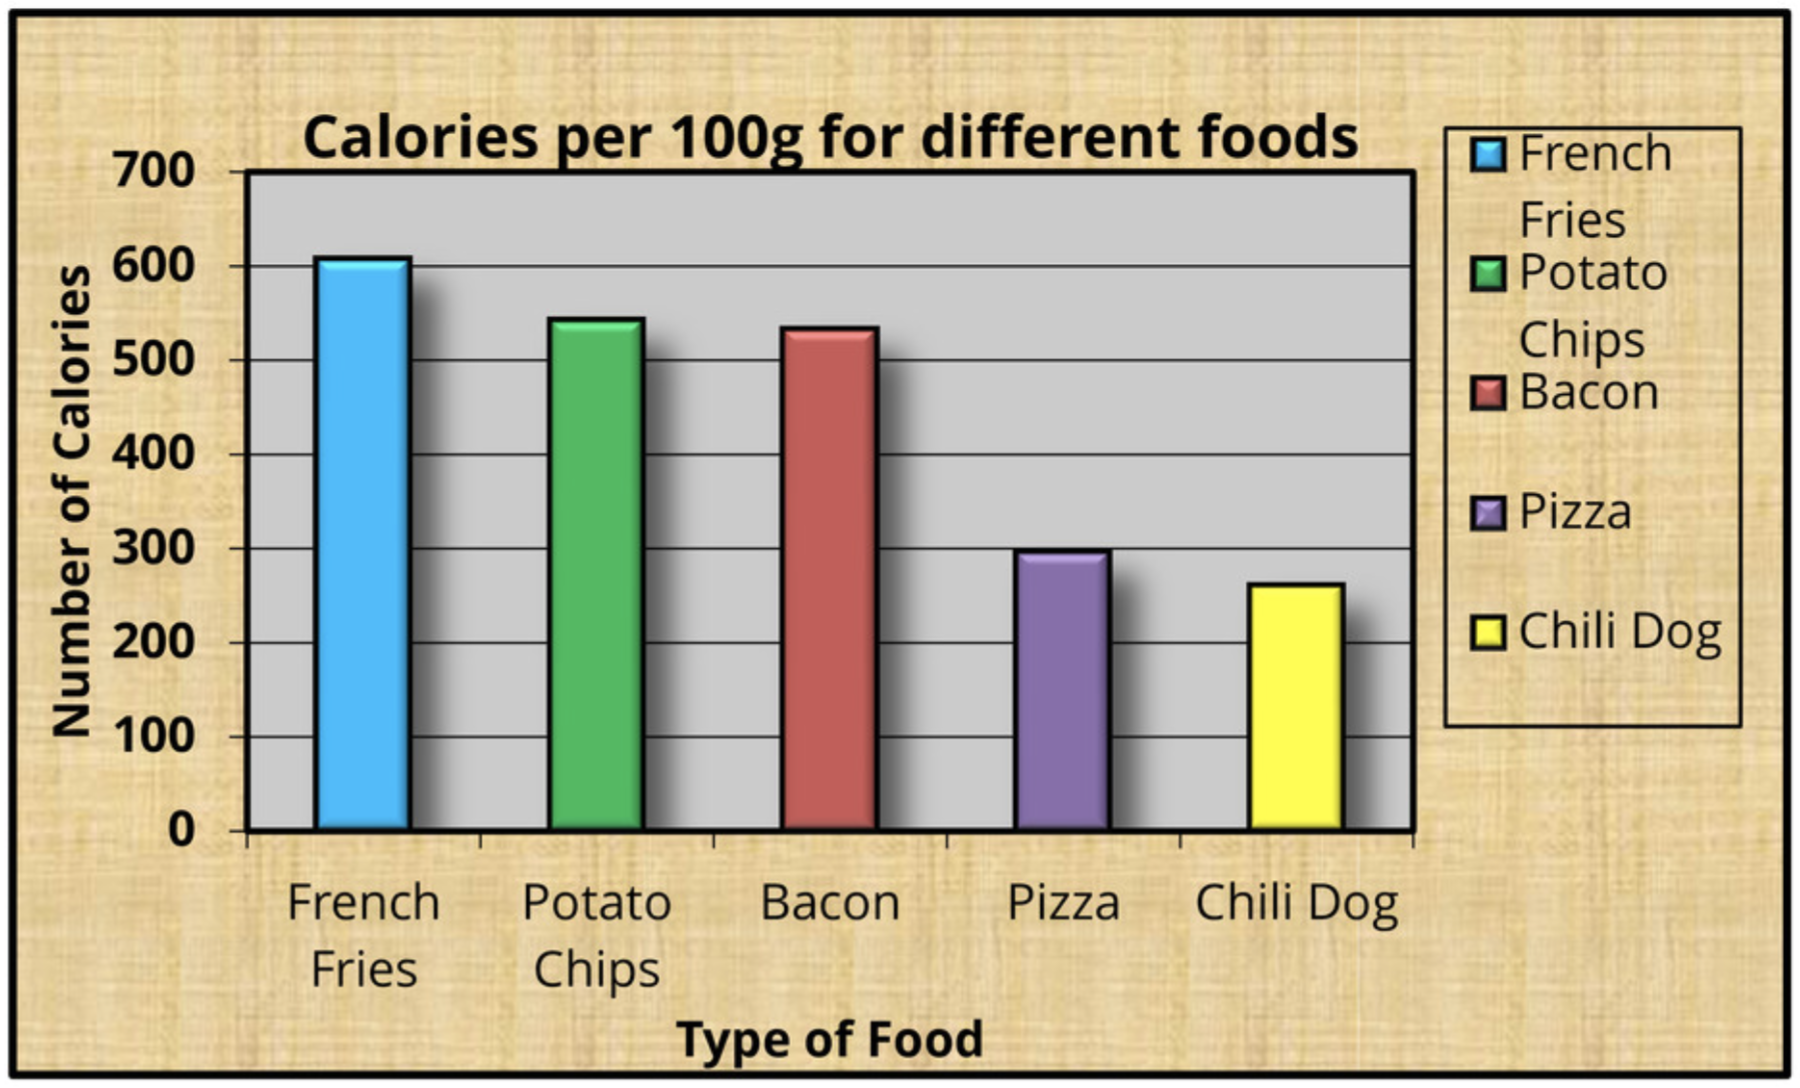
\includegraphics[width=0.48\textwidth]{barplot-before}%
\hspace{\fill}%
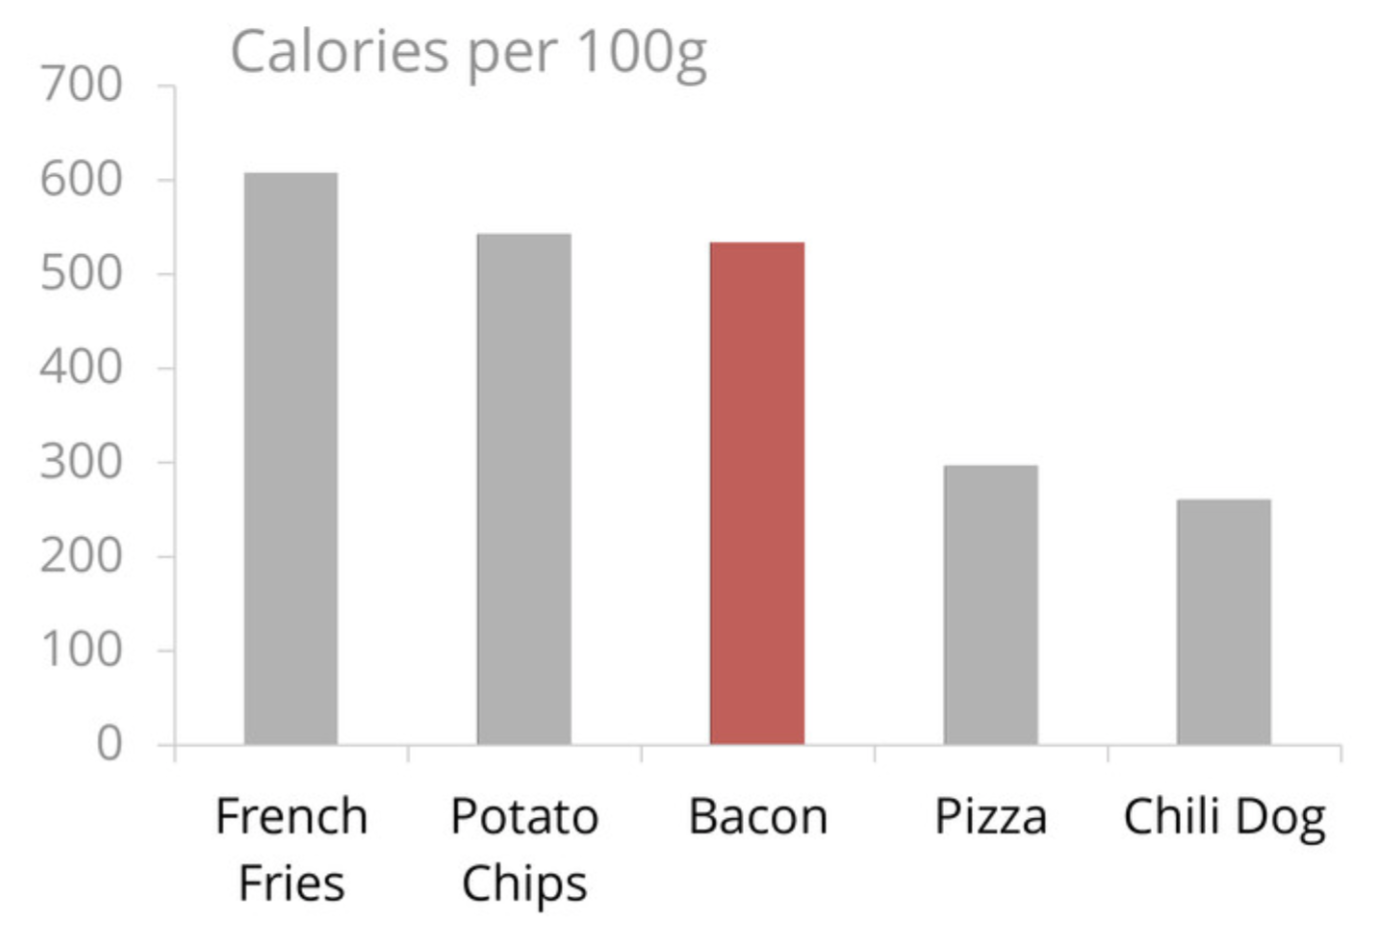
\includegraphics[width=0.48\textwidth]{barplot-after}
\sidecaption{\label{fig:barplot}%
   Removing unnecessary clutter.}[-2\baselineskip]
   % using optional last parameter: negative offset to correct vertical
   % position of caption (this caption is two lines high)
\end{figure}


Make sure that your figures work when \textbf{printed in monochrome}, i.\,e., you shouldn't rely on the colors too much. If you do use colors, use the same color palette in all figures, and ensure that readers with color blindness can differentiate all colors.

If you present plots of experimental results, use a tool that allows you to automatically \textbf{recreate plots}. To this end, you recommend to write scripts that create the plots based on raw data. Another benefit is that you will be able to change the design of all plots with little effort. Common tools are Python's \textsc{matplotlib} (also consider using \textsc{seaborn}), R's \textsc{ggplot2}, and \textsc{gnuplot}. Make sure to export your plots as PDFs.

\subsubsection{Figure Layout Options}

Place your figures in the \emph{Figures} folder. This will allow you to omit the directory name when you refer to them in the \verb|\includegraphics{filename}| command.

Putting the following code into the source file produces the picture of the electron that you can see in Fig.~\ref{fig:Electron}.
\begin{latex}
\begin{figure}[t] % place at top of page (recommended)
\centering

\includegraphics[width=0.75\textwidth]{Electron}
\decoRule
\caption[An Electron]{An electron (artist's impression).}
\label{fig:Electron}
\end{figure}
\end{latex}

\begin{figure}[t] % place at top of page (recommended)
\centering

\includegraphics[width=0.75\textwidth]{Electron}
\decoRule
\caption[An Electron]{An electron (artist's impression).}
\label{fig:Electron}
\end{figure}

Figures should appear on the page where they are referenced first or on one of the subsequent pages. The recommended \textbf{figure placement} is the top of the page (denoted by \code{[t]}). Don't worry about figures not appearing exactly where you write them in the source. Sometimes there is not enough room to fit a figure directly where it should go (in relation to the text) and so LaTeX puts it at the top of the next page.

Every figure needs a \textbf{descriptive caption and a label}. Figure captions must always appear below the included graphics file within the \code{figure} environment.

Every figure \textbf{must be referenced} in the text at least once, either in parentheses (cf. Fig.~\ref{fig:Electron}) or explicitly in the sentence: Figure~\ref{fig:Electron} shows an electron. Refer to figures using the abbreviation \code{Fig.} followed by a protected space (\verb|~|) and \verb|\ref|. Exception: write \code{Figure} if it is the first word of a sentence. Note \verb|Fig.| and \verb|Figure| are capitalized when they are used as part of a reference.

The \verb|\caption| command contains two parts,%
\marginnote{Theses at PSI usually do not have a List of Figures. You can, therefore, omit the part in square brackets.} 
the first part, inside the square brackets is the title that will appear in the \emph{List of Figures}, and so should be short.
 The second part in the curly brackets should contain the longer and more descriptive caption text.

The \verb|\decoRule| command is optional and simply puts a horizontal line below the image. Such a line can be useful with figures that are not symmetrical or whose exterior is uneven at the bottom.

Resize your figures, ideally consistently, to an appropriate size, e.\,g., a fraction of \texttt{\textbackslash textwidth}. Check that the font size (after scaling) is consistent. This advice is especially important when you include figures with different aspect ratios.

LaTeX is capable of using images in PDF, JPG, and PNG format. Using \textbf{vectorized figures} (PDF) is preferred as they usually provide sharper results at smaller file size. If you \emph{have} to use pixel graphics, create them with a sufficiently high resolution, i.\,e., at least 300 dpi.


\paragraph{Wide Figures} You can also add wide figures that span the full width of a page. These should be placed at the top of the page. The following code creates the example figure (Fig.~\ref{fig:widefig}):
\begin{latex}
\begin{figure*}[t] % place at top
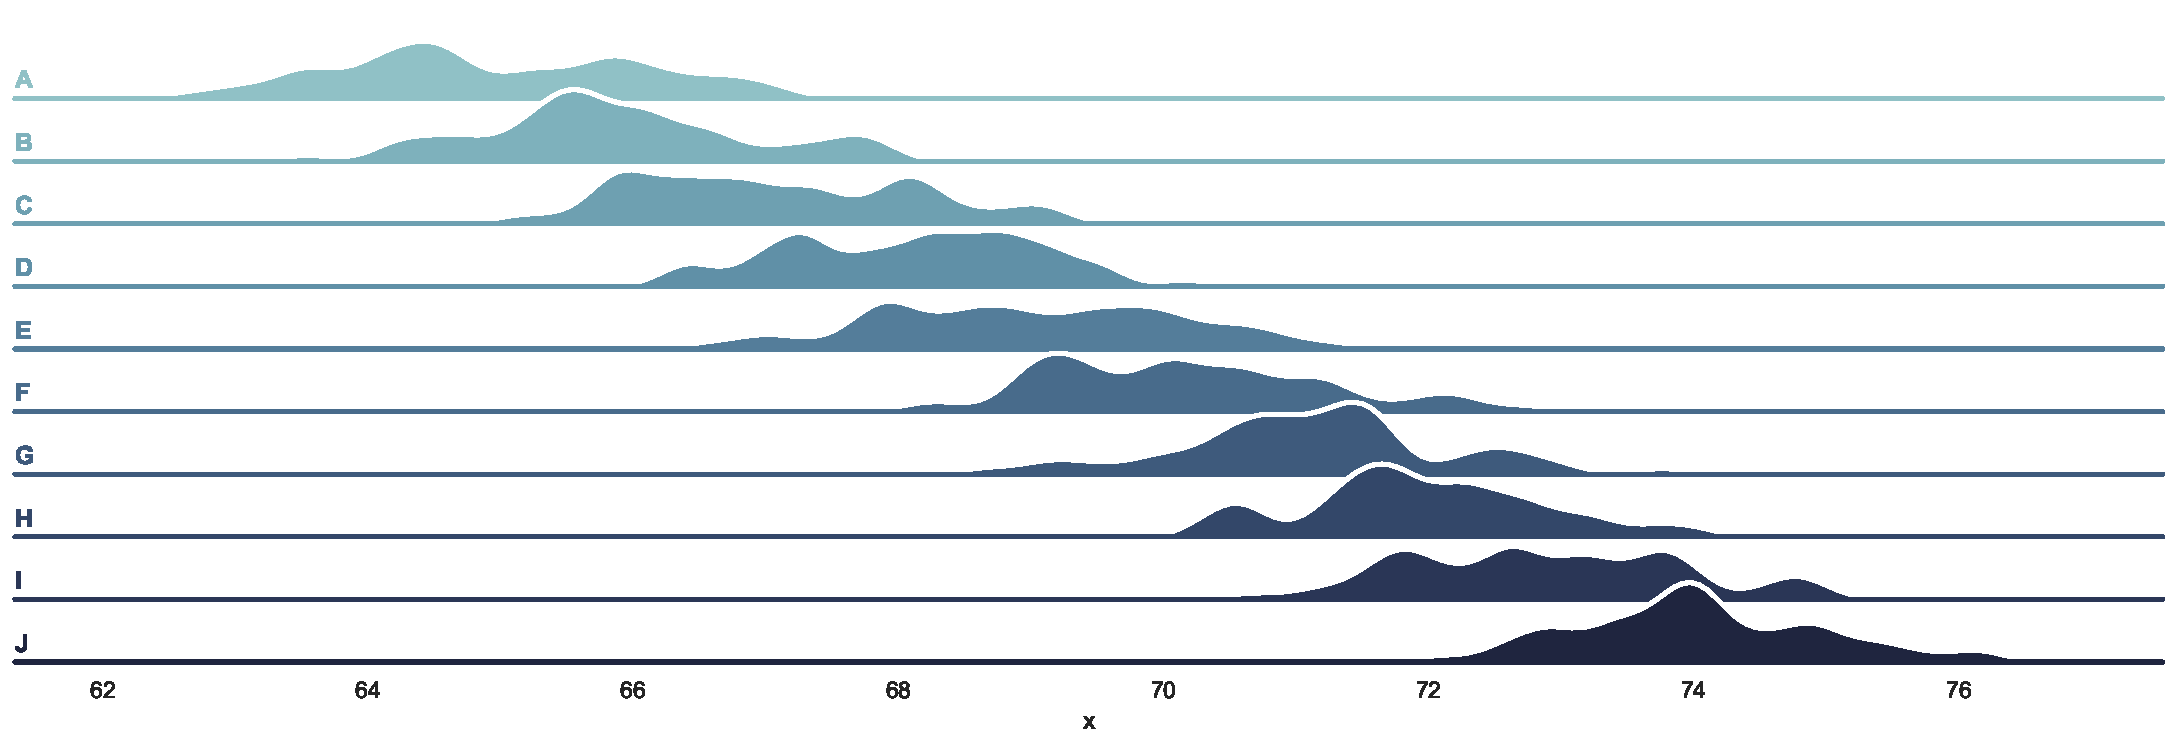
\includegraphics[width=\widefigurewidth]{plot.pdf}
\caption{\label{fig:widefig}
  This is a full-width figure. Lorem ipsum dolor sit amet, …
}
\end{figure*}
\end{latex}

\begin{figure*}[t]
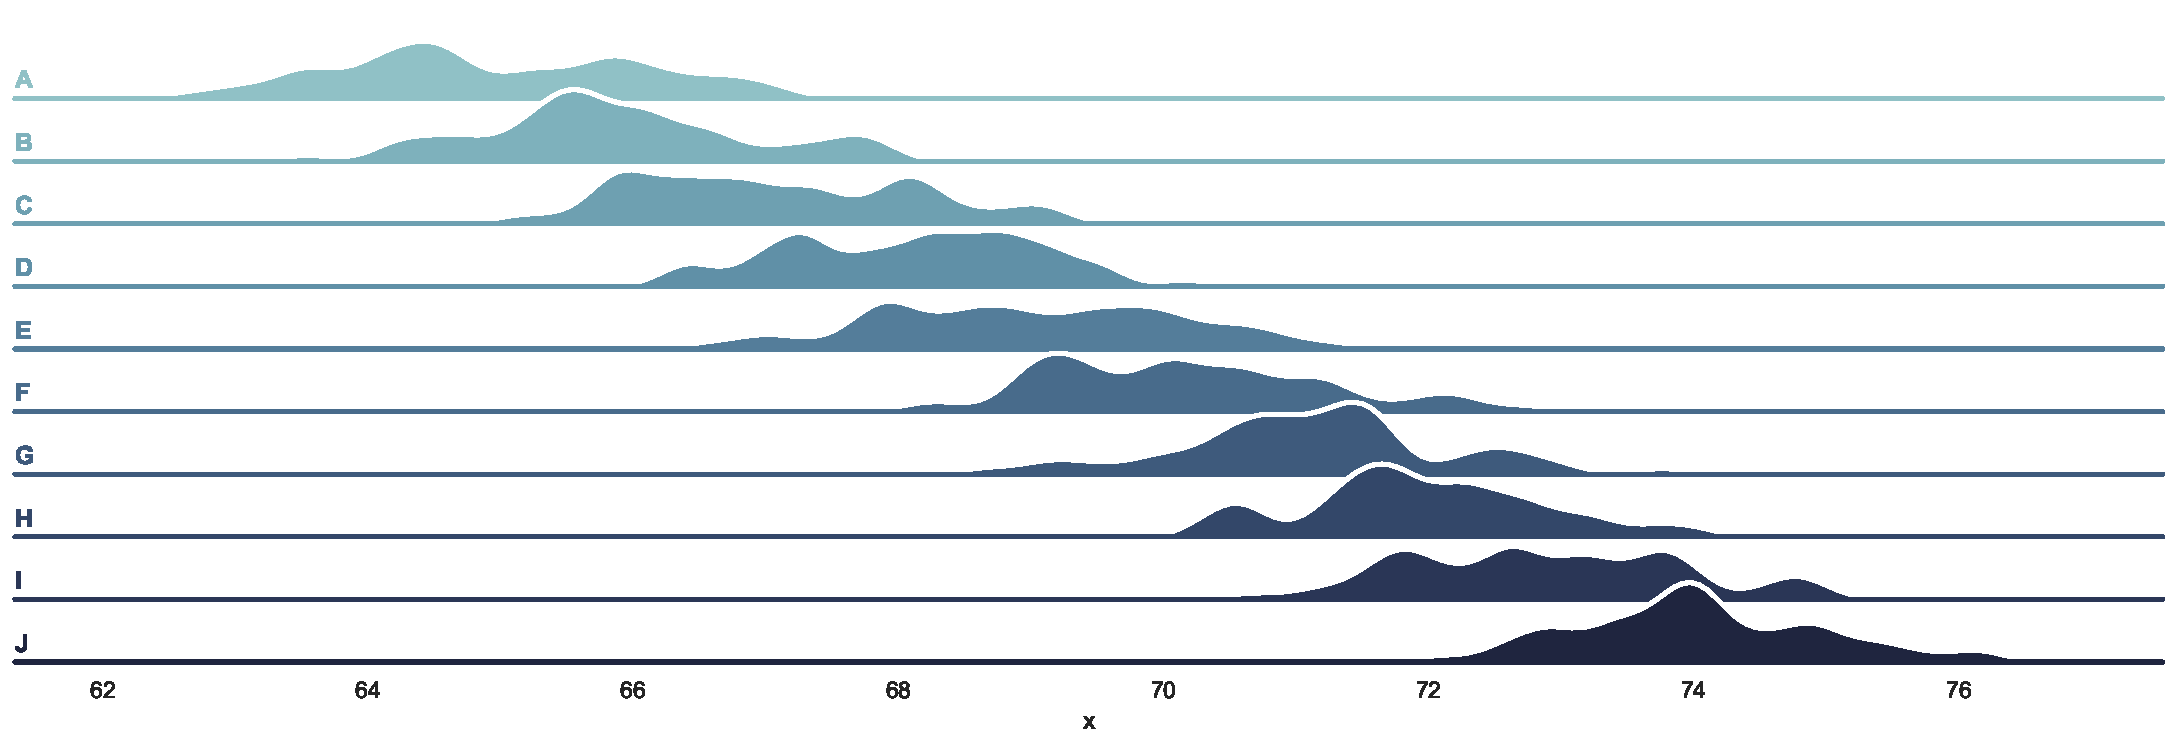
\includegraphics[width=\widefigurewidth]{plot.pdf}
\caption{\label{fig:widefig}This is a full-width figure. Lorem ipsum dolor sit amet, consectetur adipisicing elit, sed do eiusmod tempor incididunt ut labore et dolore magna aliqua. Ut enim ad minim veniam, quis nostrud exercitation ullamco laboris nisi ut aliquip ex ea commodo consequat.}
\end{figure*}


\paragraph{Side-by-Side Figures} Sometimes it is desirable to show multiple figures next to each other. There are several approaches for that, e.\,g., using the \texttt{subfigure} package. In many cases, however, a comprehensive subfigure support is not needed. A lightweight approach as shown in Fig.~\ref{fig:barplot} may be sufficient. This result is achieved with the following code:
\begin{latex}
\begin{figure}[t]
\centering
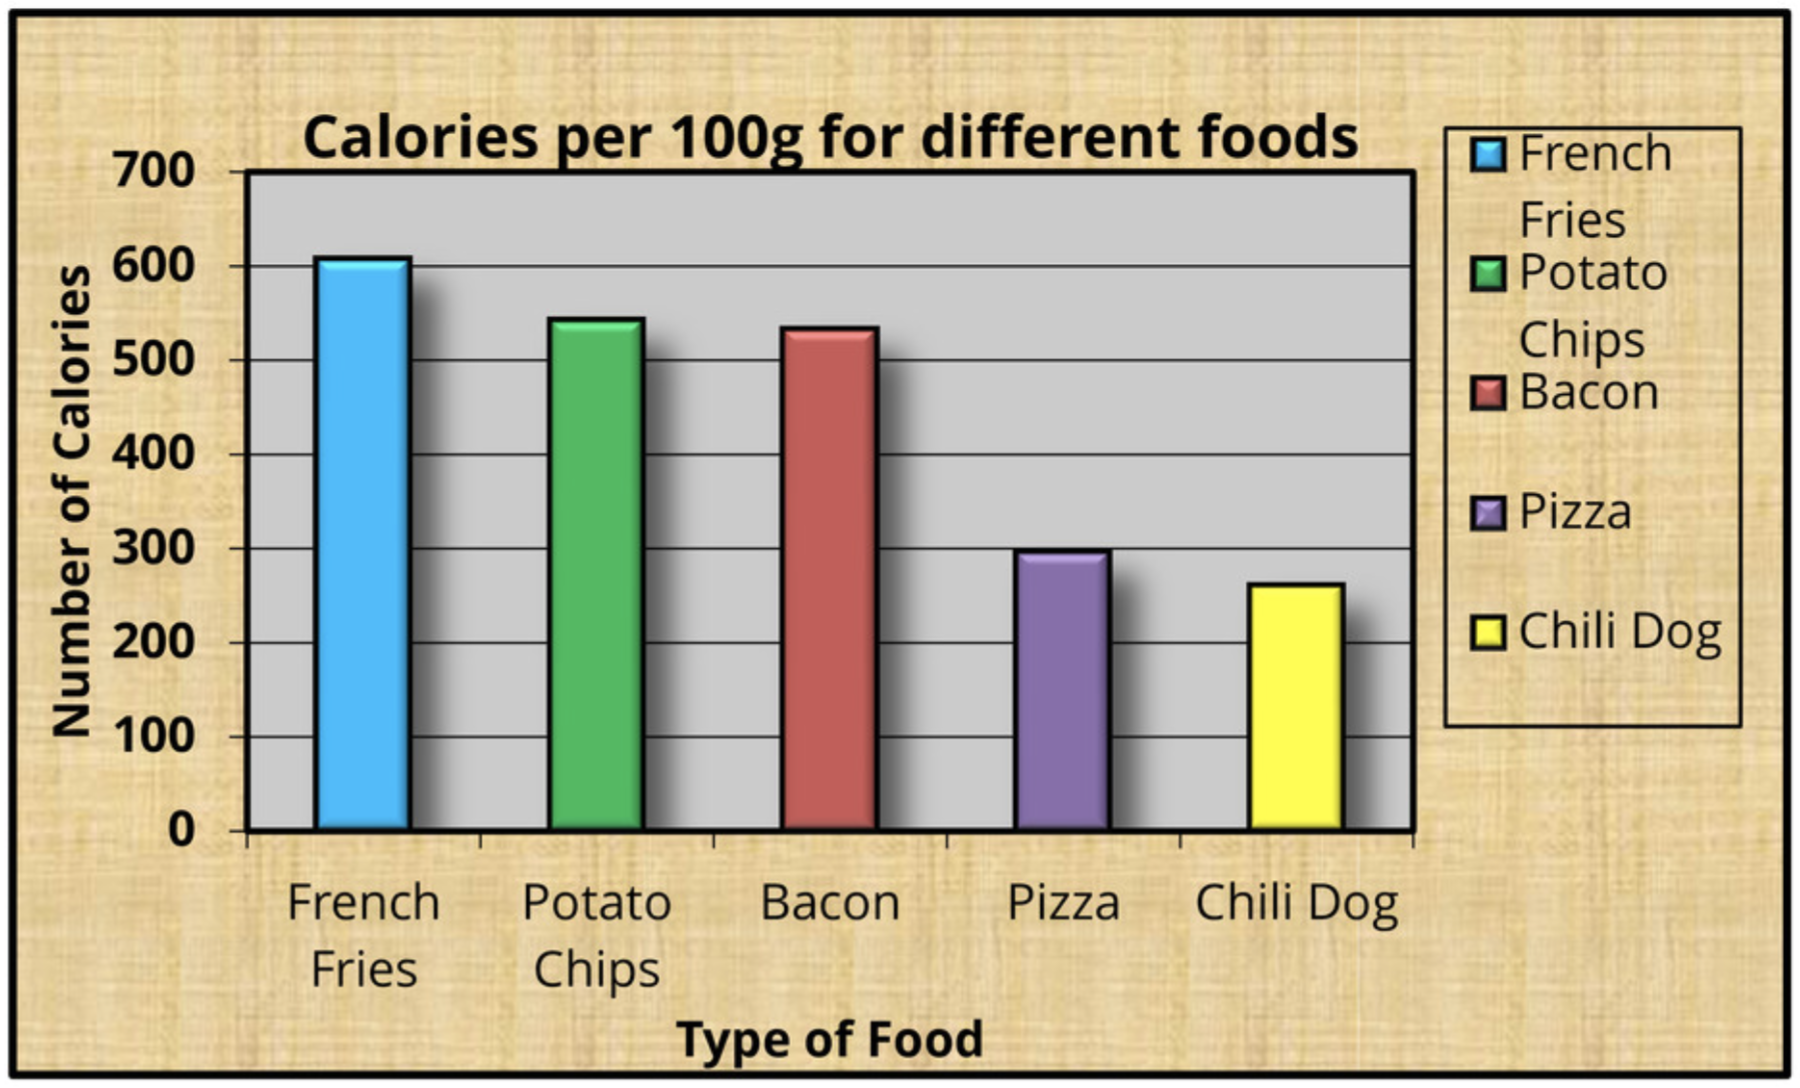
\includegraphics[width=0.48\textwidth]{barplot-before}%
\hspace{\fill}%
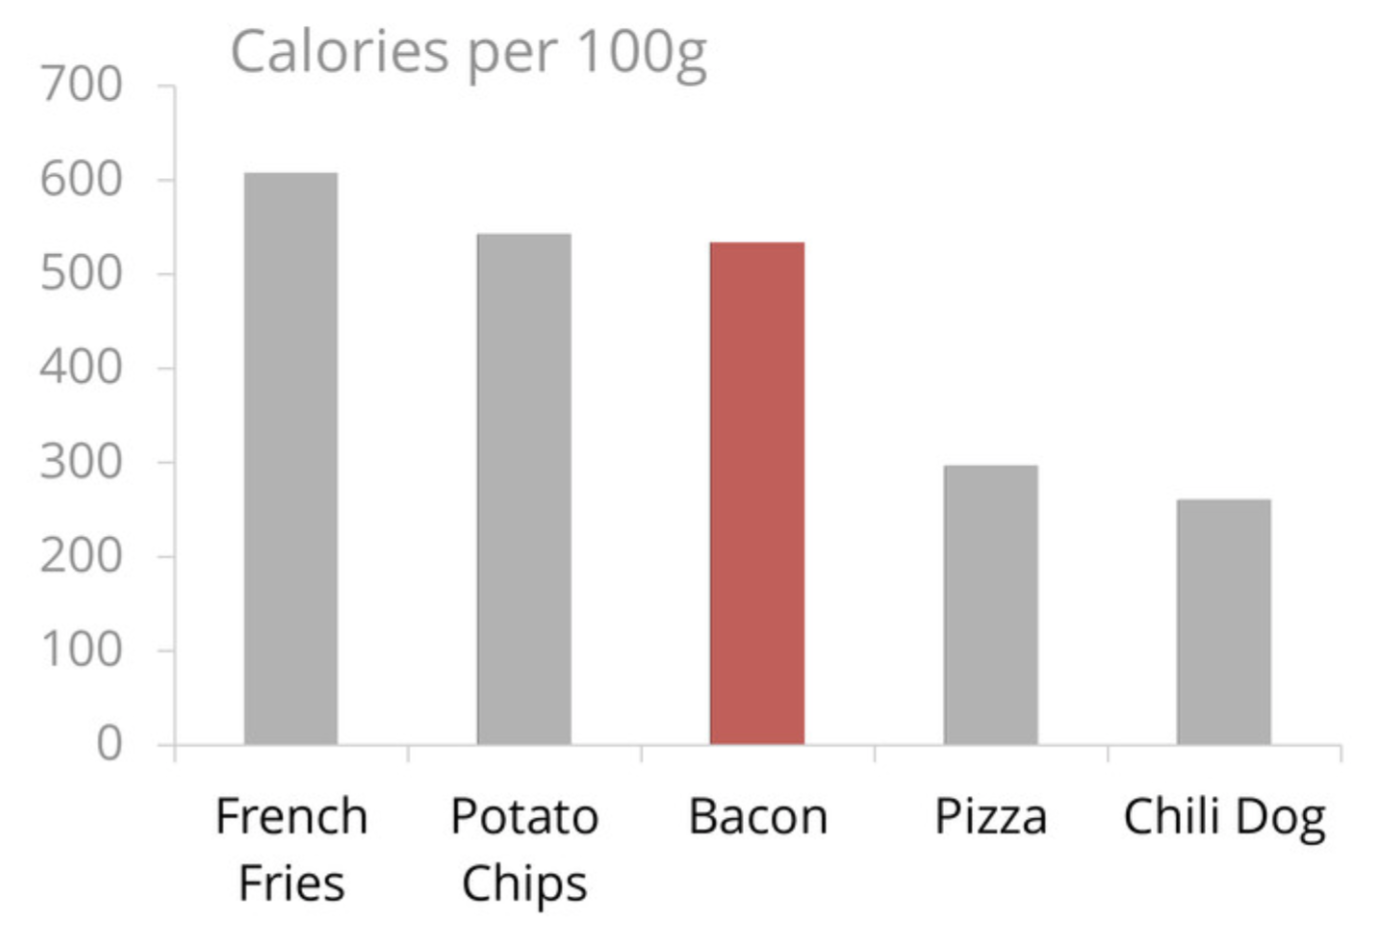
\includegraphics[width=0.48\textwidth]{barplot-after}
\sidecaption{\label{fig:barplot}%
   Removing unnecessary clutter.}[-2\baselineskip]
   % using optional last parameter: negative offset to correct vertical
   % position of caption (this caption is two lines high)
\end{figure}
\end{latex}

Figure \ref{fig:barplot} also shows how to create \textbf{captions in the margin} (\code{sidecaption}). Whether you do this or not is up to you.
Just ensure to place all captions consistently, i.\,e., either in the margin or above or below floats for tables and figures, respectively. Note that \code{sidecaption} does not work with floating listings.


\begin{marginfigure}[1\baselineskip] % move figure down by 1 line 

\includegraphics[width=\marginparwidth]{Electron}
\caption{\label{fig:marfig}This is a margin figure with a short caption.}
\end{marginfigure}

\paragraph{Margin Figures} Sometimes, it makes sense to place figures in the margin. Margin figures work best when they are simple and unobtrusive. They can be used to illustrate concepts and to visualize trends. Do not use them for figures that convey essential results.
%
You can create margin figures like Fig.~\ref{fig:marfig} with the following code:
\begin{latex}
\begin{marginfigure}[1\baselineskip] % move figure down by 1 line 

\includegraphics[width=\marginparwidth]{Electron}
\caption{\label{fig:marfig}This is a margin figure with a short caption.}
\end{marginfigure}
\end{latex}


\subsection{Listings}

If you are new to LaTeX,%
\marginnote{If you have Python, you can consider the more modern package \code{minted}, which uses {pygments} for syntax highlighting.}
we recommend to use the \emph{listings} package for code listings. With the template's default monospace font, lines can have up to 89 characters.

You can create floating listings, which behave very much like floating figures and tables, i.\,e., they have a caption and can be referenced (cf. Listing~\ref{lst:listing} for an example). Sometimes, however, the properties of floating listings are undesirable. For short code fragments, it often makes more sense to use a non-floating listing.

Listing~\ref{lst:listing} has been generated with the following code:
\begin{latex}
\begin{lstlisting}[language=Python,float=t,
  caption={This is an example of syntax highlighting of
  Python code with a relatively long caption},label={lst:listing}]
import numpy as np

test = "This is a test string"
 
def incmatrix(genl1,genl2):
    ...
    return M
\end{lstlisting}
\end{latex}

\begin{lstlisting}[language=Python,float=t,
  caption={This is an example of syntax highlighting of
  Python code with a relatively long caption},label={lst:listing}]
import numpy as np

test = "This is a test string"
 
def incmatrix(genl1,genl2):
    m = len(genl1)
    n = len(genl2)
    M = None # to become the incidence matrix
    VT = np.zeros((n*m,1), int)  # dummy variable
 
    # compute the bitwise xor matrix
    M1 = bitxormatrix(genl1)
    M2 = np.triu(bitxormatrix(genl2),1) 
 
    for i in range(m-1):
        for j in range(i+1, m):
            [r,c] = np.where(M2 == M1[i,j])
            for k in range(len(r)):
                VT[(i)*n + r[k]] = 1;
                VT[(i)*n + c[k]] = 1;
                VT[(j)*n + r[k]] = 1;
                VT[(j)*n + c[k]] = 1;
 
                if M is None:
                    M = np.copy(VT)
                else:
                    M = np.concatenate((M, VT), 1)
 
                VT = np.zeros((n*m,1), int)
 
    return M
\end{lstlisting}


\section{Mathematics}

Equations allow you to express yourself with high precision and no ambiguity. 

The \enquote{Not So Short Introduction to LaTeX} (available on \href{http://www.ctan.org/tex-archive/info/lshort/english/lshort.pdf}{CTAN}) should tell you everything you need to know for most cases of typesetting mathematics. If you need more information, a much more thorough mathematical guide is available from the AMS: \href{{ftp://ftp.ams.org/pub/tex/doc/amsmath/short-math-guide.pdf}}{A Short Math Guide to LaTeX}.

There are many different LaTeX symbols to remember, luckily you can find the most common symbols in \href{http://ctan.org/pkg/comprehensive}{The Comprehensive \LaTeX~Symbol List}.

You can write an equation, which is automatically given an equation number by LaTeX like this:
\begin{latex}
\begin{equation}
E = mc^{2}
\label{eqn:Einstein}
\end{equation}
\end{latex}

This will produce Einstein's famous energy-matter equivalence equation:
\begin{equation}
E = mc^{2}
\label{eqn:Einstein}
\end{equation}

LaTeX automatically gives all equations you write equation numbers. If you don't want a particular equation numbered, use the unnumbered form:
\begin{latex}
\[ a^{2}=4 \]
\end{latex}

You can also have equations in the middle of a paragraph, e.\,g., \( E = mc^{2} \), with this syntax: 

\begin{latex}
\( E = mc^{2} \)
\end{latex}

%----------------------------------------------------------------------------------------

\section{Structuring your Thesis}

You should break your thesis up into chapters and sections. LaTeX automatically builds a Table of Contents by looking at all the \verb|\chapter{}|, \verb|\section{}|  and \verb|\subsection{}| commands you write in the source. You may even think about using \emph{sub}subsections (\verb|\subsubsection{}|). All of these will be hierarchically numbered.

Use \textbf{(sub-)subsections} only if you use them consistently in all or at least multiple chapters. Otherwise, you should opt for a \verb|paragraph{}|, which structures pieces of content with bold non-numbered inline headings (examples throughout this guide).

\textbf{Avoid dangling elements} in the hierarchy: If you have a Section~1.1, you should also have (at least) Section~1.2. This rule applies to all levels of the hierarchy.

The Table of Contents is configured to only list \emph{chapters} and \emph{sections}. We do not recommend to include \emph{(sub-)subsections} as this results in a very long Table of Contents, which may become difficult to read. If you do want to change the depth of the Table of Contents, you can change the value \verb|\etocsettocdepth| in \file{setup.tex}.

Use \textbf{title case} in your \emph{chapters}, \emph{sections}, and \emph{paragraphs}. Consider, for instance, \url{https://capitalizemytitle.com} for title case capitalization rules.

Within a section, you should \textbf{walk the reader through your text}:
\begin{quote}
In the following, we describe the three primitives of concept X. First, X uses the Y algorithm. …

The second concept is Z …
\end{quote}

\section{Typography}

Use emphasis sparingly. This advice is especially true for \textbf{bold print} (\verb|\textbf{bold print}|). Resist the urge to use it in the main text; use \emph{italics} (\verb|\emph{italics}|) instead.

Note, however, that \textbf{too frequent use of italics} can also be annoying.%
\marginnote{See also \href{https://sblhs2.com/2016/09/15/italics-scare-quotes/}{Italics or Scare Quotes?}} 
We recommend using it to emphasize ordinary words that are used as special terms – and only at its first occurrence. Also, you should emphasize words that you would stress when reading aloud, indicating that they are especially relevant for the meaning.


Generally, we recommend \textbf{avoiding scare quotes}.%
\marginnote{See \href{https://style.mla.org/quotes-when-nothing-is-being-quoted/}{Quotes When Nothing Is Being Quoted}}
Some authors use scare quotes to signal that they are using a word in a non-standard, ironic, or otherwise special sense (cf. Chicago Manual of Style). Scare quotes convey an informal tone. Moreover, they cause ambiguity, as the reader cannot be sure about the intention of the author.

You should split your content into \textbf{proper paragraphs} by adding empty lines between adjacent blocks of text in the source file. Using a mixture of paragraphs and line breaks, which you could create with \verb|\\| at the end of a line, is strongly discouraged because this practice creates a noisy layout.

Use \textbf{thin spaces} (\verb|\,|) in the appropriate places. For instance, write \verb|i.\,e.,| to obtain i.\,e. (pronunciation: ``that means''). The same applies to e.\,g. (pronunciation: ``for example''). These two abbreviations are normally followed by a comma in American English.

\textbf{Dashes} can be used instead of colons or pairs of commas to mark off a nested clause. Use an \emph{en dash} for that purpose -- like in this example. If you cannot type an \emph{en dash} on your keyboard, you can write two regular hyphens next to each other. LaTeX will substitute them with an \emph{en dash}. While we have no strict preference, we recommend using \emph{en dashes} instead of the longer \emph{em dashes}.

Use en dashes also for ranges, e.\,g., when you write something like 5--10\,\% (note the thin space before the \% symbol).

Use a proper \textbf{minus symbol} (e.\,g., by using math mode like this \(-1.337\)). Also, use a sensible number of digits after the decimal point.

Use proper \textbf{directional quotation marks} like ``these.'' Directional quotation marks are created  \verb|``like this''|, by using \verb|\enquote{text}|, or by copy-and-pasting the respective Unicode characters. Note that in contrast to conventions in the German language, the closing quotation mark is placed \emph{after} any subsequent punctuation, e.\,g., ``like this,'' and ``like that.''

\paragraph{Further Reading}

If you speak German, consider reading \textsc{typokurz} (\url{https://zvisionwelt.wordpress.com/downloads/}), a short introduction to typographic issues. You can also browse Matthew Butterick's website \url{https://practicaltypography.com}.

\section{Language and Style}

Language issues distract readers from the content and make it difficult to assess its merits. You should, therefore, pay close attention to language and style.

\subsection{Spelling, Hyphenation, and Grammar}

Ensure correct spelling throughout your text. Check your writing with a spell checker. There are special spellcheckers for LaTeX, but copy-and-pasting the text into Word may also be an option.

Ensure proper hyphenation throughout your text. You will have to intervene, for instance, when words extend into the margin of the page (creating so-called overfull hboxes). You can override LaTeX's hyphenation rules by inserting \verb|\-| into a word. This special character indicates a conditional hyphenation point.

It makes sense to define hyphenation rules globally. To this end, place custom hyphenation definitions like \verb|\hyphenation{FORTRAN Hy-phen-a-tion}| after the \verb|\begin{document}| clause.
\todo[noline]{Oh no, an overful hbox!}
The example definition prevents any hyphenation of the word FORTRAN and defines three hyphenation points for the word Hyphenation.

Also, check your text for common grammar issues (cf. Sect.~\ref{sec:style}).

\subsection{Style}
\label{sec:style}

This section contains selected pieces of advice on particular aspects and typical errors. For a more comprehensive treatment, we refer the reader to the paragraph \nameref{par:commonbugs} at the end of this section.

The main goal of a thesis is to convey information without ambiguity. Write concisely and use a simple language. Avoid complex sentence structures, unnecessary words, and unnecessarily complicated words. A thesis is not the place to show off your mastery of grammar and vocabulary. There are various (mostly web-based and commercial) tools that can help you identify common issues in your text.\footnote{We are aware of \url{https://grammarly.com}, \url{https://languagetool.org}, \url{http://www.hemingwayapp.com} as well as the command-line tool Academic-Writing-Check (\url{https://github.com/devd/Academic-Writing-Check}).}


\subsubsection{The Science of Scientific Writing}

Even if a text uses a simple language, it may be difficult to read, because it does not convey the writer's train of thoughts coherently. In short, your goal is to connect every sentence explicitly to its predecessor – which is, of course, easier said than done.

A good resource to develop this skill is the article \emph{The Science of Scientific Writing} by George D. Gopen and Judith A. Swan.\footnote{The article can be obtained from \url{https://cseweb.ucsd.edu/~swanson/papers/science-of-writing.pdf} and \url{https://www.americanscientist.org/blog/the-long-view/the-science-of-scientific-writing}} 
The advice from this article is also part of the three lessons on scientific writing offered by Duke University.\footnote{Homepage of the lessons: \url{https://cgi.duke.edu/web/sciwriting/}, PDF slides: \url{https://cgi.duke.edu/web/sciwriting/resources/201108_DukeScientificWritingWorkshop.pdf} (these URLs could not be archived).}

The remainder of this section contains selected excerpts from \emph{The Science of Scientific Writing}. Consider reading the original article for a more extended treatment, including worked examples.

\paragraph{Subject-Verb Separation (Excerpts)}

  Readers expect a grammatical subject to be followed immediately by the verb. Anything of length that intervenes between subject and verb is read as an interruption, and therefore as something of lesser importance.
The reader’s expectation stems from a pressing need for syntactic resolution, fulfilled only by the arrival of the verb. Without the verb, we do not know what the subject is doing, or what the sentence is all about.

As a result, the reader focuses attention on the arrival of the verb and resists recognizing anything in the interrupting material as being of primary importance.
The longer the interruption lasts, the more likely it becomes that the “interruptive” material actually contains important information; but its structural location will continue to brand it as merely interruptive.
Unfortunately, the reader will not discover its true value until too late – until the sentence has ended without having produced anything of much value outside of the subject-verb interruption.

\paragraph{The Stress Position (Excerpts)}

It is a linguistic commonplace that readers naturally emphasize the material that arrives at the end of a sentence. We refer to that location as a “stress position.”
Beginning with the exciting material and ending with a lack of luster often leaves us disappointed and destroys our sense of momentum.

The stress position can change in size from sentence to sentence. Sometimes it consists of a single word; sometimes it extends to several lines. The definitive factor is this: The stress position coincides with the moment of syntactic closure. A reader has reached the beginning of the stress position when she knows there is nothing left in the clause or sentence but the material presently being read.

To summarize the principles connected with the stress position, we have the proverbial wisdom, “Save the best for last.”

\paragraph{The Topic Position (Excerpts)}

To summarize the principles connected with the other end of the sentence, which we will call the topic position, we have its proverbial contradiction, “First things first.”
In the stress position the reader needs and expects closure and fulfillment; in the topic position the reader needs and expects perspective and context.

The information that begins a sentence establishes for the reader a perspective for viewing the sentence as a unit: Readers expect a unit of discourse to be a story about whoever shows up first. “Bees disperse pollen” and “Pollen is dispersed by bees” are two different but equally respectable sentences about the same facts. The first tells us something about bees; the second tells us something about pollen. In fact, “Pollen is dispersed by bees” is the superior sentence if it appears in a paragraph that intends to tell us a continuing story about pollen. Pollen’s story at that moment is a passive one.

Readers also expect the material occupying the topic position to provide them with linkage (looking backward) and context (looking forward).

\subsubsection{Selected Syntactical Conventions}

Avoid using \textbf{informal contractions} such as \emph{can't}, \emph{don't}, and \emph{it's}. Replace them with \emph{cannot}, \emph{do not}, and \emph{it is}.

We recommend using the \textbf{serial comma} in all lists to avoid ambiguity. The serial comma is also known as the \emph{Oxford comma}: Insert  it right before the word \emph{and} that leads the last item of a list. The following example illustrates the benefit of using a serial comma:\footnote{Source: \url{https://nhigham.com/2016/02/16/the-serial-or-oxford-comma/}}
\begin{quote}
  Three important techniques in the design of algorithms are bisection, divide and conquer, and recursion.
\end{quote}

Use \textbf{bullet lists} correctly. ``Lists are common in all forms of writing. The list items can be included within the text or put on separate lines. Separate lines are used in order to draw attention to the items, to ease reading when the items are long or numerous, or to facilitate cross-reference to specific items.''\footnote{Source: \url{https://nhigham.com/2015/12/17/punctuating-lists/}} The environments \code{itemize} and \code{enumerate} produce lists on separate lines. It is considered good style to use punctuation in such a way that the lists form full sentences if their items were \emph{not} split into separate lines. One way to achieve this goal is to only put full sentences into the list. If list items, however, are sentence fragments, additional punctuation is necessary (example taken from source mentioned in footnote):

\begin{quote}
  We used three different algorithms in the experiments. The table reports the performance of
\begin{itemize}
\item Algorithm 3.1 (based on a Taylor series),
\item Algorithm 3.2 (with parameter \(k = 1\)), and
\item Algorithm 3.3 (with tolerance \(10^{-8}\)).
\end{itemize}
\end{quote}

\paragraph{Common Bugs in Writing}
\label{par:commonbugs}
Read the comprehensive list of common bugs in writing by Henning Schulzrinne, which is available at \url{http://www.cs.columbia.edu/~hgs/etc/writing-bugs.html}.

\section{Concluding Remarks}

Scientific work and writing are skills that you can practice. Seminar papers serve that purpose during the studies. The final thesis shows which methodical and technical skills you have acquired. In addition to proper time management, discipline, and willingness to research literature, communication with one's supervisor is the key to success.

\paragraph{Further Reading}

This guide is not meant to cover all topics of scientific writing in detail. Consider the very comprehensive document \emph{Scientific Writing for Computer Science Students} by Wilhelmiina Hämäläinen (\url{http://www.cs.joensuu.fi/pages/whamalai/sciwri/sciwri.pdf}). Hämäläinen has collected a substantial amount of advice with a particular focus on English grammar and the peculiarities of computer science.

There is also an abundant number of books on scientific writing. We can recommend the following:
\begin{itemize}
\item M. Alley. The Craft of Scientific Writing; and
\item W. Strunk and E.B. White. The Elements of Style.
\end{itemize}

Finally, if you seek inspiration, we recommend to read these reports by well-known scientists:
\begin{itemize}
\item Randy Pausch: Time Management (\url{http://www.youtube.com/watch?v=oTugjssqOT0}),
\item Richard Hamming: You and Your Research (\url{http://www.cs.virginia.edu/~robins/YouAndYourResearch.html}), and
\item Nick Feamster: Writing Tips for Academics (\url{http://greatresearch.org/2013/10/11/storytelling-101-writing-tips-for-academics/}).
\end{itemize}

The remaining parts of this guide contain less-often needed technical details and historical information about the template as well as a loose collection of assorted advice.
%\include{Chapters/Chapter3}
%\include{Chapters/Chapter4}
%\include{Chapters/Chapter5}


%----------------------------------------------------------------------------------------
%	THESIS CONTENT - APPENDICES
%----------------------------------------------------------------------------------------

\appendix % Cue to tell LaTeX that the following "chapters" are Appendices

%%% CHANGES NEEDED HERE
% 
% Include the appendices of the thesis as separate files from the Appendices folder
% Uncomment the lines as you write the Appendices

% Appendix A
 
\chapter{More Information About the Template}

\section{Template Features}\label{ThesisFeatures}

\subsection{Printing Format}

\marginnote{At the PSI Chair, we highly encourage you to use double-sided printing.}This thesis template is designed for double-sided printing (i.\,e., content on the front and back of pages) as most theses are printed and bound this way. Switching to one-sided printing is as simple as uncommenting the \option{oneside} option of the \code{documentclass} command at the top of the \file{main.tex} file. You may then wish to adjust the margins to suit specifications from your institution.

The headers for the pages contain the page number on the outer side (so it is easy to flick through to the page you want) and the chapter name on the inner side.

The text is set to 11 point by default with single line spacing,\marginnote{For a thesis at the PSI Chair, stick with the defaults.} again, you can tune the text size and spacing should you want or need to using the options at the top of \file{main.tex}. The spacing can be changed similarly by replacing the \option{singlespacing} with \option{onehalfspacing} or \option{doublespacing}.

\subsection{Using US Letter Paper}

\marginnote{For a thesis at the PSI Chair, stick with the defaults.}
The paper size used in the template is A4, which is the standard size in Europe. If you are using this thesis template elsewhere and particularly in the United States, then you may have to change the A4 paper size to the US Letter size. This can be done in the margins settings section in \file{main.tex}.

Due to the differences in the paper size, the resulting margins may be different to what you like or require (as it is common for institutions to dictate certain margin sizes). If this is the case, then the margin sizes can be tweaked by modifying the values in the same block as where you set the paper size. Now your document should be set up for US Letter paper size with suitable margins.

\subsection{References}

The \code{biblatex} package is used to format the bibliography and inserts references such as this one \parencite{murdoch_steven_j._chip_2010}. The options used in the \file{main.tex} file mean that the in-text citations of references are formatted with the author(s) initials and the year \cite{anderson_ross_emv:_2014} of the publication. Multiple references are separated by semicolons (e.\,g., \cite{solat_security_2017, bond_chip_2014}). This is done automatically for you. To see how you use references, have a look at the \file{Chapter1.tex} source file. Reference managers allow you to simply copy and paste or drag references into the document.

The bibliography is typeset with references listed in alphabetical order by the first author's last name. This is similar to the APA referencing style. To see how LaTeX typesets the bibliography, have a look at the very end of this document (or just click on the reference number links in in-text citations).

\paragraph{BibTeX Backend}

As the ``old'' \code{bibtex} backend does not correctly handle unicode character encoding (i.\,e., ``international'' characters), we use the more modern \code{biber} BibTeX engine in this template.

Here, we cite a lot of references so that the list of references gets populated \cite{murdoch_steven_j._chip_2010,anderson_ross_emv:_2014,kou_weidong_secure_2003,solat_security_2017,bond_chip_2014,ortiz_s._is_2006,haselsteiner_security_2006,galloway_visa_2019,zhou_nshield_2014,lalehTaxonomyFraudsFraud2009,ferradiWhenOrganizedCrime2016,Yang10,Kopsell06,VilaGM03,Herrmann12-ipv6prefix,Herrmann14-diss,HBF:2013,Herrmann11-NordSec,AcarEEJND14,Herrmann09,WangG13,Raymond00,Hintz02,Herrmann14-encdns,Goodson12-privacy,WendolskyHF07,chaum81,BertholdFK00,Dingledine04,rfc5246,LoesingMD10,FuchsHF13}.


\section{History of this Template}
The template has been adapted from \file{MastersDoctoralThesis.cls}, which was obtained from \url{https://www.latextemplates.com/template/masters-doctoral-thesis}. The template has its own \emph{document class}, which is defined in \file{PSIThesis.cls} file.

The MastersDoctoralThesis LaTeX thesis template is originally based and created around a LaTeX style file created by Steve R.\ Gunn from the University of Southampton (UK), department of Electronics and Computer Science. You can find his original thesis style file at his site, here
\url{http://www.ecs.soton.ac.uk/~srg/softwaretools/document/templates/} (link not available any more).

Steve's \file{ecsthesis.cls} was then taken by Sunil Patel who modified it by creating a skeleton framework and folder structure to place the thesis files in. The resulting template can be found on Sunil's site here:
\url{http://www.sunilpatel.co.uk/thesis-template}

Sunil's template was made available through \url{http://www.LaTeXTemplates.com} where it was modified many times based on user requests and questions. Version 2.0 and onwards of this template represents a major modification to Sunil's template and is, in fact, hardly recognisable. The work to make version 2.0 possible was carried out by \href{mailto:vel@latextemplates.com}{Vel} and Johannes Böttcher.

%% Appendix B
 
\chapter{Further Recommendations}

This section contains further recommendations, which our students found useful in the past.

\section{Introduction Chapter}

Don’t be boring! Pull in the reader with a peculiar observation or a surprising result of your thesis.

Approaches to structure your introduction:
\begin{itemize}
\item Start with the general, close with the specific.
\item Start with what is already well-known, move on to what has only recently become known.
\item State the objective of the thesis, then describe your approach.
\end{itemize}

End the introduction with a paragraph \emph{Outline of the Thesis} that describes its structure in prose.

\section{Related Work Chapter}

Think about a story and which message you want to convey. Some common themes are:
\begin{itemize}
\item “It used to be a difficult problem, but we know how to solve it.”
\item “While a lot of proposals exist, none has gained traction in reality. X found that one of the primary reasons for that situation is …”
\item “The field is a cat-and-mouse game between refined attacks and defenses. A common theme is … and overlooked areas are …”
\item “While most of the current literature focuses on X, it would make sense to apply techniques from field Y to the problem. One could then refine the problem as …”
\end{itemize}

\section{Conclusion Chapter}

A basic recipe for a conclusion chapter:
\begin{itemize}
\item a summary,
\item a critical assessment of what you have achieved,
\item pointers to related other topics,
\item a statement of the impact of the results, and
\item pointers to future work.
\end{itemize}

\section{Thesis Length}

Typical theses range from 25 to 100 pages. Do not worry too much about the page count. Write everything that is necessary to assess and reproduce your work, but no more. Less is more!

Check the individual parts for an appropriate length: Do not write five pages in the introduction if the main part has only 15 pages.


\section{Practices to Avoid}

\begin{itemize}
\item Colloquial style: “Computation power has skyrocketed in the last few years.”
\item Widespread knowledge: “The Internet is becoming more and more important.”
\item Superlatives: “One of the most beautiful concepts”, “great possibilities.”
\item Be careful with strong claims: “the only possibility”, “the best solution”, “impossible.”
\end{itemize}
%\include{Appendices/AppendixC}


%----------------------------------------------------------------------------------------
%	BIBLIOGRAPHY
%----------------------------------------------------------------------------------------

% Bibliography has no wide margins:
\newgeometry{
	inner=2cm, % Inner margin
	outer=2cm, % Outer margin
	marginparwidth=0cm,
	marginparsep=0mm,
	bindingoffset=.5cm, % Binding offset
	top=1.5cm, % Top margin
	bottom=2.5cm, % Bottom margin,
	includehead,
	includefoot
	% showframe, % Uncomment to show how the type block is set on the page
}

\addchap{References}

% allow much more liberal line breaks in URLs
\setcounter{biburllcpenalty}{7000}
\setcounter{biburlucpenalty}{8000}

% adjust space between key and entry, default is 2\labelsep
\setlength{\biblabelsep}{1\labelsep} 

% configures indentation of bibentries
\defbibenvironment{bibliography}
  {\list
     {\hspace{0.5\labelalphawidth}\bfseries\printtext[labelalphawidth]{%
        \printfield{prefixnumber}%
        \printfield{labelalpha}%
        \printfield{extraalpha}}}
     {\setlength{\labelsep}{\biblabelsep}%
      \setlength{\leftmargin}{0.5\labelalphawidth}%
      \setlength{\itemsep}{1.5\bibitemsep}%
      \setlength{\parsep}{\bibparsep}}%
      \renewcommand*{\makelabel}[1]{##1\hss}}
  {\endlist}
  {\item}

% enables two-column layout for bibliography
\setlength\columnsep{2em}
\begin{multicols}{2}
	\begin{refcontext}[sorting=nyt] % sort bibliography by last name, year, title
		\renewcommand*{\bibfont}{\small\RaggedRight}
		\linespread{1.0}\selectfont % increase linespread if desired (not recommended)
		\printbibliography[heading=none]
	\end{refcontext}
\end{multicols}

%----------------------------------------------------------------------------------------

%----------------------------------------------------------------------------------------
%	DECLARATION PAGE
%----------------------------------------------------------------------------------------

\begin{declaration}
\addchaptertocentry{\authorshipname} % Add the declaration to the table of contents

%\selectlanguage{ngerman}
Ich erkläre hiermit gemä\ss\ \S~17 Abs.\,2 APO, dass ich die vorstehende {\abschluss}arbeit selbständig\\ verfasst und keine anderen als die angegebenen Quellen und Hilfsmittel benutzt habe.

\bigskip
\bigskip

\begin{tabular}{@{}l@{}}
  Bamberg, den \rule[-0.8em]{10em}{0.5pt}\\[2ex]
  ~
\end{tabular}
\hspace{\fill}%
\begin{tabular}{@{}c@{}}
  \rule[-0.8em]{20em}{0.5pt}\\[2ex]
  \authorname 
\end{tabular}\hspace{\fill}




\end{declaration}

\end{document}
